%\documentclass[brudnopis,xodstep]{kdypl}%% opcja 'brudnopis' zwraca stopkę z nr wersji pracy i e-mailem, opcja 'xodstep' zwiększa odstęp do 1.3
% klasa posiada opcję 'licencjacka' dla prac licencjackich oraz 'magisterska' dla prac magisterskich

\documentclass[licencjacka]{kdypl}
\usepackage[T1]{fontenc}
\usepackage[utf8]{inputenc}
\usepackage[MeX]{polski}
\usepackage{graphicx}
\graphicspath{{Grafika/}}
\usepackage{caption}
\usepackage{color}
\bibliographystyle{papalike}
\usepackage[round,sort&compress]{natbib}
\providecommand{\BIBand}{i}
\usepackage{indentfirst}
\usepackage{float}
\usepackage{booktabs}
\usepackage{subfig}

%% Spis rzeczy
%\usepackage{makeidx}
%\makeindex






\usepackage[breaklinks]{hyperref}
\hypersetup{colorlinks,citecolor=black,filecolor=black,linkcolor=black,urlcolor=black}


\captionsetup[figure]{font=footnotesize}



% Opcjonalnie identyfikator dokumentu (drukowany tylko
% z włączoną opcją `brudnopis'):
\nrwersji {1}

% Dane autora(ów):
\author{Robert Tarnas}
\nralbumu{402178}
\email{robert.tarnas@protonmail.com}

%Do oświadczenia:
\autor{Robert Tarnas}

% Tytuł pracy:
\title{Neuroestetyczna analiza iluzji wzrokowych. Przypadek sztuki op-art'u}%tytuł polski
\tytulang{Neuroaesthetical analysis of optical illusions in op-art paintings}

%Do oświadczenia:
\tytul{Neuroestetyczna analiza iluzji wzrokowych. Przypadek sztuki op-art'u}

% Kierunek:
\kierunek {Kognitywistyka}

% Rok obrony:
\date {2019}

% Jeżeli nie podano miejsca zostanie wpisany `Poznań'
\miejsce {Poznań}

% Tytuł naukowy, imię i nazwisko promotora, np.:
%  dr Jan Kowalski
%  prof. dr hab.~Jan Kowalski
% itp.
\opiekun  {dr hab. Piotr Przybysz}

%wyodrebnienie cytatu kursywą.
\newenvironment{itquote}
{\begin{quote}\itshape}
{\end{quote}}



%zmiana sposobu numerowania w spisie tresci

\renewcommand\thechapter{\arabic{chapter}}
\renewcommand\thesection{\arabic{section}}


\begin{document}

%%Polskie
\begin{abstract}
\noindent%Jeśli streszczenie składa się z jednego akapitu (a raczej powinno)

Neuroestetyka jest interdyscyplinarnym programem badawczym poświęconym badaniu reakcji estetycznych powstających podczas obcowania ze sztuką. Początki badań estetycznych sięgają XIX-wiecznej psychologii eksperymentalnej, a dokładniej jej pobocznego nurtu – estetyki eksperymentalnej Gustava T. Fechnera. Współcześnie neuroestetyka opiera się głownie na neuroobrazowaniu pracy mózgu podczas wykonywania zadań percepcyjnych związanych z oceną estetyczną. Tematem pracy jest przedstawienie aktualnego stanu badań nad iluzjami wzrokowymi w sztuce. Analizę iluzji wzrokowych opieram na współczesnych pracach naukowych poświęconych psychologi widzenia. Inspiracją do napisania pracy była chęć pokazania zjawiska iluzji optycznych jako środka wyrazu w ramach obecnego we współczesnym malarstwie nurtu op-art. Pracę wieńczy przegląd i analiza iluzji wzrokowych, wykorzystywanych przez Mauritsa Cornelisa Eschera.

\end{abstract}

\keywords{sztuka optyczna, M.C Escher, malarstwo, iluzje optyczne, op-art, neuroestetyka}

%%Angielskie
\begin{abstracteng}
\noindent%Jeśli streszczenie składa się z jednego akapitu (a raczej powinno)

Neuroaesthetics is interdisciplinary research programme, focused on studying aesthetic emotions, created in the process of perception of art. Neuroaesthetic originate from research began in XIX century, firstly conducted by experimental psychology, or more specifically in its secondary branch – experimental aesthetics of Gustav T. Fechner. Today, neuroaesthetics prefer more modern approach. The scientists are focused on using neuroimaging machinery \& software to conduct their modern experiments. The topic of this thesis concerns usage of optical illusion in the visual art. The general idea in this thesis was to analyze works of Dutch painter – M.C Escher in the op-art movement of modern art.


\end{abstracteng}

\keywordseng{optical art, M.C Escher, paintings, optical illusions, op-art, neuroaesthetics}

\maketitle




\tableofcontents \thispagestyle{empty}
\chapter*{Wstęp}\addcontentsline{toc}{chapter}{Wstęp}


Neuroestetyka jest interdyscyplinarnym programem badawczym poświęconym badaniu reakcji estetycznych, powstających podczas obcowania ze sztuką. Początki badań estetycznych sięgają XIX-wiecznej psychologii eksperymentalnej, a dokładniej jej pobocznego nurtu -- estetyki eksperymentalnej Gustava T. Fechnera. Współcześnie neuroestetyka wykorzystuje metody neuroobrazowania funkcji i struktur mózgu podczas przeprowadzania eksperymentów percepcyjnych związanych z oceną estetyczną  \citep{Bremer}.

Praca podzielona jest na trzy rozdziały. W rozdziale pierwszym przedstawione są założenia neuroestetycznego programu badań nad sztuką oraz przykłady klasycznych badań z~neuroestetyki, wraz z omówieniem różnych prób zdefiniowania dzieła sztuki podejmowanych w ramach tej dziedziny nauki. Rozszerzam definicję neuroestetyczną dzieła sztuki o ujęcie fenomenologiczne dzieła sztuki malarskiej Romana Ingardena. 

Rozdział drugi przedstawia mechanizmy powstawania iluzji i ich wpływ na układ wzrokowy. Przedstawiono tam definicję bodźca iluzyjnego, podział iluzji wzrokowych według Jana Młodkowskiego oraz różne przykłady iluzji występujące w literaturze.


Rozdział trzeci krótko przedstawia nurt sztuki optycznej w malarstwie współczesnym. Artyści tworzący w nurcie op-art chętnie wykorzystują iluzje wzrokowe w swoich pracach. Jednym z takich artystów jest holenderski grafik Maurits Cornelis Escher.  Modyfikuje on perspektywę oraz kształty przedmiotu, aby przedstawić dzieło sztuki jako obiekt wieloznaczny, będący rodzajem zagadki percepcyjnej. Analiza dzieł Eschera została przeprowadzona w oparciu o trójpoziomowy semiotyczny model dzieła sztuki Moniki Bianki Florek.


\chapter{Dzieło sztuki w ujęciu neuroestetycznym i fenomenologicznym}\label{r1}

\section{Założenia neuroestetycznego programu badań nad sztuką}

Sztuka od zawsze wzbudza spore zainteresowanie naukowców, filozofów i historyków sztuki. Próbują oni zrozumieć w jaki sposób postrzeganie obrazu czy słuchanie muzyki może powodować powstawanie przeżyć estetycznych. Przez lata sądzono, że przeżycia estetyczne wymykają się poznaniu naukowemu, ale wątpliwości te postanowiła rozwiać nowa dziedzina nauki -- \textit{neuroestetyka,} proponująca naukowe podejście do badania piękna i przeżyć estetycznych.

Neuroestetyka jest interdyscyplinarnym programem badawczym zajmującym się odkrywaniem podłoża zjawisk składających się na szeroko pojęte poznanie estetyczne. Neuroestetyka łączy dokonania m.in. historii sztuki, filozofii, psychologii, neurobiologii i neurofizjologii w jeden program badawczy. Neuroestetycy zakładają, że wszystkie przeżycia jakich doznajemy podczas obcowania i tworzenia sztuki można wyjaśnić w sposób naukowy. Dokonać tego można na wiele różnych sposobów, m.in. poprzez identyfikacje neuronalnych korelatów doświadczenia piękna, sformułowanie szeregu praw odpowiadających za percepcję sztuki, które byłyby uniwersalne i niezależne od uwarunkowań kulturowych, a także poprzez opisanie emocji towarzyszących spostrzeganiu obiektów uznawanych za piękne \citep[s. 112]{przybysz2016}. Dzieło sztuki jest w~neuroestetyce traktowane specjalnie, jako przedmiot szczególnie wyróżniający się z otoczenia, pełniący funkcję silnego bodźca pobudzającego zmysły. Artysta dla neuroestetyków jest nieświadomym neurobiologiem, który nie ma akademickiej wiedzy na temat tego jak działa mózg, ale potrafi ją nieświadomie wykorzystywać \citep[s. 19]{neurobiolog}. 

Źródłem wiedzy dla neuroestetyków jest sam mózg osoby kontemplującej sztukę. Dlatego też inspiracji dla współczesnych badań neuroestetycznych należy poszukiwać w XIX-wiecznej psychologii eksperymentalnej, a zwłaszcza w badaniach prowadzonych przez jedną z jej najstarszych odmian -- \textit{estetykę eksperymentalną} Gustava T. Fechnera.\footnote{Sam Fechner razem z Wilhelmem Wundtem i Hermannem von Helmholtzem jest uważany za prekursora podejścia eksperymentalnego w psychologii \citep[s. 11]{Bremer}.} Zasadniczą różnicą pomiędzy podejściem Fechnera, a tradycyjnie rozumianą \textit{estetyką}, która należy do dyscyplin filozoficznych, jest nacisk na badania eksperymentalne, stanowiące podstawową metodę weryfikacji teorii naukowych \citep[s. 11]{Bremer}. Niektóre z odkryć Fechnera wydają się interesujące również dziś. Podczas serii eksperymentów w 1860 roku, Fechner wykazał, że niektóre proporcje i formy abstrakcyjne są bardziej atrakcyjne od innych. Podejmował również próby sformułowania uniwersalnych zasad powstawania przeżyć estetycznych. Wyróżnił między innymi, zasadę \textit{progu estetycznego,} mówiącą o tym, że spostrzegane przeżycie musi być odpowiednio silne żeby wywołać reakcję, czy \textit{stopniowania estetycznego,} którą określał jako obecność jak największej ilości łącznie występujących wrażeń \citep[s. 11-12]{Bremer}.

Sposób prowadzenia badań jest obecnie zupełnie różny od metod, które były w użyciu w XIX stuleciu. Współcześnie bardzo dużą uwagę przykłada się do metod neurobrazowania mózgu, które pozwalają obserwować aktywność mózgu podczas wykonywania jakiegoś zadania poznawczego. Jednym z częściej używanych narzędzi jest \textit{funkcjonalny rezonans magnetyczny (fMRI)}. Za jego pomocą można wyszczególnić te obszary mózgu, które są zaangażowane w konkretne zadanie poznawcze podczas eksperymentu. Mierzy on sygnał wynikający z  różnicy stężeń utlenowanej i odtlenowanej hemoglobiny. Przewaga krwi utlenowanej w danej strukturze mózgu świadczy o większym jej zaangażowaniu w zadanie \citep[s. 55]{Jaskowski}.
\section{Koncepcja dzieła sztuki jako obiektu deformacyjnego}

Istnieje wiele pomysłów na to jak można współcześnie badać powstawanie przeżyć estetycznych, jedną z nich jest koncepcja dzieła sztuki jako obiektu deformacyjnego Vilayanura Ramachandrana i Williama Hirsteina. Proponują oni aby na dzieło sztuki patrzeć jak na \textit{superbodziec\footnote{Autorami pojęcia superbodźca są Konrad Lorenz i jego uczeń Niko Tinbergen, którzy w latach 1950-1951 prowadzili eksperymenty z pisklętami mewy morskiej \citep{tinbergen}.},} którego zadaniem jest pobudzenie układu percepcyjnego odbiorcy. Dzieło sztuki jest bodźcem specjalnym, zdolnym do wywołania trzech różnych reakcji organizmu składających się na odbiór estetyczny. Są to:
\begin{enumerate}
\item Skupienie uwagi widza,
\item Odrzucenie konwencjonalnego odbioru dzieła,
\item Wywołanie emocji estetycznej
(Za: \citealt[s. 370]{Przybysz2006}).
\end{enumerate}

Artyści, często nieświadomie, wyolbrzymiają cechy obrazowanego przedmiotu, starając się uwypuklić jedną kluczową dla niego cechę. Dzięki temu przedmiot realny staje się w istocie karykaturą, ale  potrafi przyciągnąć i zainteresować sobą odbiorce dzieła \citep[s. 333]{Rama}.
Wyolbrzymianie cech może odbywać się w różnych przestrzeniach, np. koloru, kształtu, postawy anatomicznej i innych (por. rys. 1.1) \citep[s. 333-335]{Rama}.

\begin{figure}[hbt]
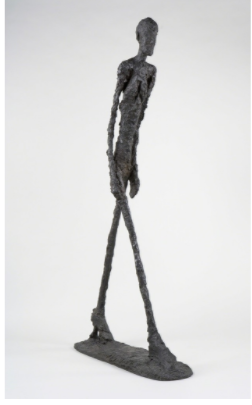
\includegraphics[width= 0.3\textwidth]{man}
\centering
\caption{Alberto Giacometti, Walking Man I, 1960. Przykład deformacji w przestrzeni kształtu (sylwetki). Rzeźba znajduje się na terenie Yuz Museum w Szanghaju. Źródło: \url{https://www.artsy.net/artwork/alberto-giacometti-walking-man-i}}
\end{figure}
\clearpage
Ramachandran z Hirsteinem uważają, że zabiegi stosowane przez artystów silnie oddziałują na odbiorcę. Żeby wyjaśnić dlaczego tak się dzieje, zaproponowali dwa niezależne wyjaśnienia: psychologiczne oraz neurologiczne \citep[s. 334-335]{Rama}. Wyjaśnienie psychologiczne opiera się na tzw. \textit{zasadzie przesunięcia szczytowego.} Opiera się ona na następującej obserwacji: ludzie i zwierzęta lepiej odpowiadają na bodźce wyolbrzymione, ponieważ takie przedmioty lepiej odróżniają się od otoczenia. System wzrokowy jest naturalnie przystosowany do spostrzegania różnic, a wszelkie kształty różniące się od przeciętnych lepiej zapadają w pamięć \cite[s. 334]{Rama}.

Drugim rodzajem wyjaśnienia jest wyjaśnienie neurologiczne. Sprowadza się ono do założenia, że istnieją w mózgu neurony odpowiedzialne za wykrywanie istotnych różnic między obiektami. Z~czysto biologicznego punktu widzenia ma to sens, ponieważ rozsądnie jest dostrzec drapieżnika lub potencjalnego partnera na tyle wcześnie aby uniknąć zagrożenia lub skorzystać z okazji. Rola artysty sprowadza się tutaj do tego żeby nie tylko dobrze ukazać obiekt, ale także wyolbrzymić jego najbardziej istotne cechy. W rezultacie otrzymuje się superbodziec, który przyciąga uwagę odbiorcy \citep[s. 335]{Rama}.




\section{Badania Zekiego nad przetwarzaniem barw}

Semir Zeki jest z wykształcenia neurobiologiem, profesorem na \textit{University College of London}, a także autorem pojęcia \textit{neuroestetyka}, które zostało użyte po raz pierwszy w roku 1995, podczas jednego z jego wykładów. Od tego czasu dziedzina znacznie się rozrosła i ciągle zdobywa zainteresowanie nowych badaczy z całego świata \citep[s. 10]{Znak}. Zeki swoim głównym obszarem zainteresowania uczynił układ wzrokowy, ponieważ jest to dominujący zmysł dla wszystkich naczelnych, w tym także i człowieka. Swoje początkowe badania prowadził na makakach królewskich (rezusach), małpach zamieszkujących tereny południowej Azji. Zeki twierdzi, że inspiracją do podjęcia badań właśnie na makakach był fakt, że ich kora wzrokowa pod względem organizacji bardzo przypomina ludzką \citep[s. 8]{Znak}. Badania przeprowadzał za pomocą mikroelektrod, które wszczepiał w mózgi małp i obserwował, które rejony mózgu są najbardziej zaangażowane w odpowiedź na określony rodzaj bodźca prezentowanego małpie \citep{Artysta}. Badania Zekiego wykazały, że kora wzrokowa makaków królewskich nie jest obszarem jednorodnym -- składa się z różnych części, z~których każda realizuje inną funkcję.\footnote{Podobną specjalizację obserwuję się także w ludzkim mózgu.} Niektóre grupy komórek mózgu reagują tylko na kolor określonego rodzaju, inne na specyficzny kształt, a jeszcze inne reagują wyłącznie na percepcję ruchu, wyładowując się zawsze wtedy kiedy spostrzegamy ruch w określonym kierunku, niezależnie od tego jaki konkretnie obiekt się porusza.\footnote{Zeki tę właściwość komórek nerwowych nazwał \textit{abstrahowaniem} tych cech obiektu, na które dana grupa neuronów jest wrażliwa \citep[s. 27]{Zeki}.} Obszarem odpowiadającym za spostrzeżenie koloru jest pole V4 w korze wzrokowej\footnote{Mikroświadomość koloru jest generowana w obrębie kompleksu V4 zasilanego przez plamki w obszarze V1 i wąskie paski w obszarze V2, których aktywność jest wymagana do stworzenia prawidłowej reprezentacji barwy w obszarze V4 \citep[s. 428]{Wieloznacznosc}.}, jego uszkodzenie powoduje \textit{achromatopsję,} czyli ślepotę na  barwy, która uniemożliwia nie tylko spostrzeganie barwy, ale udaremnia wszystkie próby jej wyobrażenia sobie. Z kolei za percepcję ruchu odpowiada pole V5 w korze wzrokowej, a jego uszkodzenie powoduje niemożność spostrzegania ruchu -- \textit{akinetopsję} \citep{Artysta}.
Odkrycia Zekiego pozwoliły również potwierdzić, że kolor i ruch w mózgu nie tylko są odrębnie spostrzegane, ale także osobno doświadczane. W jednym z eksperymentów zespół Zekiego wyświetlał badanym czerwone i zielone prostokąty umieszczone na czarnym tle, które w krótkich odstępstwach czasowych poruszały się na przemian w górę i w dół. Wnioski z tego eksperymentu są zaskakujące -- osoby badane nie wiązały danego koloru z odpowiadającym mu ruchem, ale tym, który nastąpił około 80 - 120 milisekund wcześniej. Oznacza to, że mózg nie czeka aż wszystkie ośrodki skończą przetwarzać dostępne im dane, ale tworzy świadomą reprezentację na bieżąco, jedynie aktualizując ją o nowe informacje w razie potrzeby \citep{Artysta}. 
Wymienione wyżej specjalne obszary w mózgu wzrokowym Zeki nazywa \textit{węzłami (nodes).} Są to obszary odpowiedzialne za przetwarzanie informacji w mózgu wzrokowym \citep[s. 426]{Wieloznacznosc}. Stanowią one integralną część szlaku wzrokowego. Jeśli informacja z danego węzła jest w danej chwili przetwarzana świadomie, to staje się on \textit{węzłem podstawowym}. Świadomościowy korelat będący rezultatem aktywności w węźle podstawowym Zeki nazywa \textit{mikroświadomością}\footnote{Węzeł podstawowy to węzeł, którego aktywność staje się elementem percepcji bez konieczności dalszego przetwarzania \citep[s. 81]{Zeki}.} \citep[s. 81]{Zeki}.
Węzły dobrze obrazują strukturę układu wzrokowego mózgu. Sygnały z~siatkówki docierają najpierw do pierwszorzędowej kory wzrokowej (V1) gdzie są przetwarzane przez specjalne komórki, zajmujące się wyodrębnianiem określonego atrybutu z sygnału. Następnie sygnał z obszaru V1 trafia do pozostałych wyższych ośrodków: V2, V4 i V5, które są zwrotnie  połączone z obszarem V1 i stale wymieniają z nim informacje.
Poniższa lista przedstawia obszary wyszczególnione przez Zekiego (por. rys. 1.5 i rys. 1.6). 



\begin{itemize}
\item Obszar V1 -- powstaje tutaj pierwotny szkic widzianego obrazu, 
\item Obszar V3 -- znajdują się tutaj komórki reagujące na kształty,
\item Obszar V4 -- zawiera komórki reagujące na kolor,
\item Obszar V5 -- znajdują się tu komórki wrażliwe na ruch i położenie przestrzenne, 
(Za: \citealt[s. 426-429]{Wieloznacznosc}).
\end{itemize}



\begin{figure}[H]
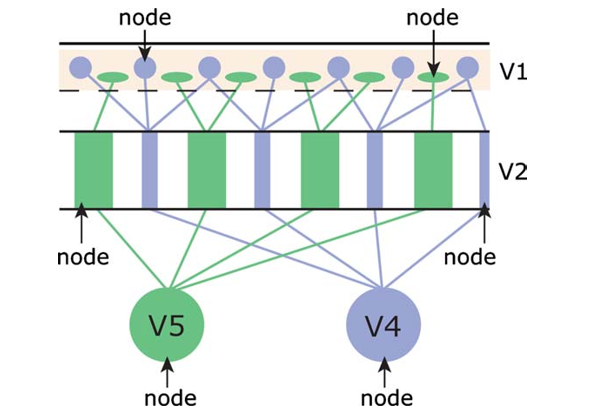
\includegraphics[width=0.7\textwidth]{wezel}
\centering
\caption{Grafika przedstawia sposób w jaki węzły wymieniają się danymi między sobą. Węzły z warstw wyższych są zwrotnie połączone z węzłami z warstwy niższej. Sygnały związane z kolorem (niebieski) i ruchem (zielony) docierają do pierwszorzędowej kory wzrokowej(V1) i obszaru przylegającego do niej (V2). Wyspecjalizowane segmenty tych obszarów wysyłają połączenia do dalszych obszarów V4 i V5, które po otrzymaniu sygnału z poprzednich węzłów stają się węzłami kluczowymi, a odebrany przez nie sygnał nie wymaga dalszego przetwarzania. (Za: \citealt[s. 426]{Wieloznacznosc}).}
\end{figure}

\begin{figure}[H]
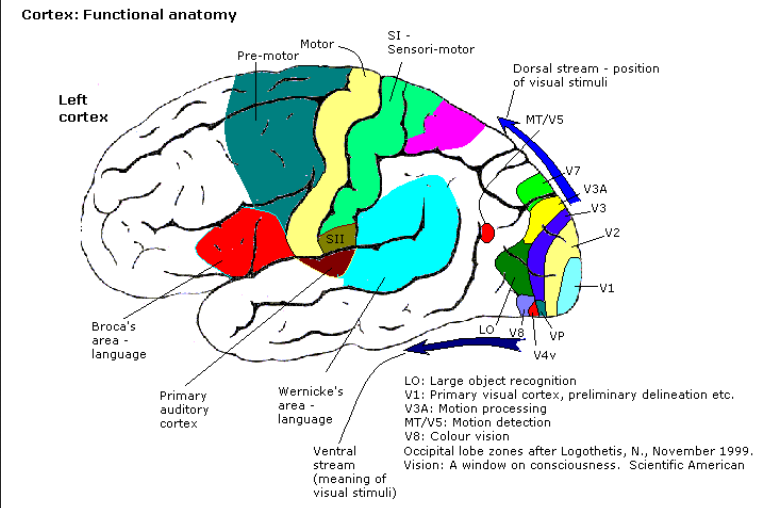
\includegraphics{brain2.png}
\caption{Mózg w ujęciu strukturalnym i funkcjonalnym. Źródło: \url{https://upload.wikimedia.org/wikipedia/commons/d/db/Constudproc.png}}
\centering
\end{figure}




\section{Dzieło sztuki jako bodziec wieloznaczny}

Późniejsze badania Zekiego dotyczyły przede wszystkim tego w jaki sposób u ludzi przebiega percepcja obiektów, których reprezentacja umysłowa nie jest stała.\footnote{Nie tworzą stałego i niezmiennego perceptu.} Obiekty takie nazywa się \textit{figurami wieloznacznymi.} Zeki określa wieloznaczność jako pewność wielu równie prawdopodobnych interpretacji, które stale konkurują ze sobą, a mózg nigdy nie jest całkowicie pewien, która z nich jest prawdziwa.\footnote{Jest to sytuacja niekorzystna dla mózgu, który dąży do stworzenia jednej, dominującej reprezentacji spostrzeganego obiektu (prawo stałości) \citep[s. 424-425]{Wieloznacznosc}}

Istnieją zatem obiekty jednoznaczne, które dla mózgu są proste w interpretacji, dwuznaczne, które potrafią wywołać dwa równoważne sobie sposoby interpretacji oraz te wieloznaczne, charakteryzujące się wielością rozwiązań, stanowiące dla mózgu spory problem, którego niejednokrotnie nie można rozwiązać. Dla mózgów osób zdrowych jednoznaczne jest widzenie barwne, ponieważ mózg, zgodnie z prawem stałości, wytwarza jedyną dopuszczalną reprezentację danego koloru, pomimo tego, że jego spostrzeżenie może przebiegać w różnych warunkach, a fala świetlna docierająca do oczu ma niejednokrotnie różną długość \citep[s. 85-86]{Zeki}.

Interesującym przykładem bodźca wieloznacznego jest \textit{trójkąt Kanzisy.} Trójkąt Kanzisy to złudzenie optyczne opisane po raz pierwszy przez włoskiego psychologa Gaetano Kanzisę w 1955 roku. Przedstawia ono figurę wieloznaczną złożoną z trzech czarnych kół, pośrodku których pojawia się biały trójkąt równoboczny, choć w rzeczywistości nie jest on narysowany \citep[s. 434]{Wieloznacznosc}. Według Zekiego to, że większość osób spostrzega tam akurat trójkąt jest rezultatem tego, że taki układ linii pobudza obecne w korze wzrokowej komórki wrażliwe na orientację przestrzenną\footnote{Znajdują się one w większości w obszarze V3 a także częściowo w wyspecjalizowanych strefach obszarów V1 i V2 \citep[s. 434]{Wieloznacznosc}}. Wykazują one silną pobudliwość na jeden, preferowany przez siebie układ linii, nie reagując w żaden sposób na przykład na linie o orientacji prostopadłej co narzuca określony kierunek interpretacji. Figury złudne takie jak trójkąt Kanzisy aktywują też obszar bocznej kory potylicznej odpowiedzialnej za rozpoznawanie przedmiotów (por. rys. 1.4) \citep[s. 86-87]{Zeki}.
\begin{figure}[H]
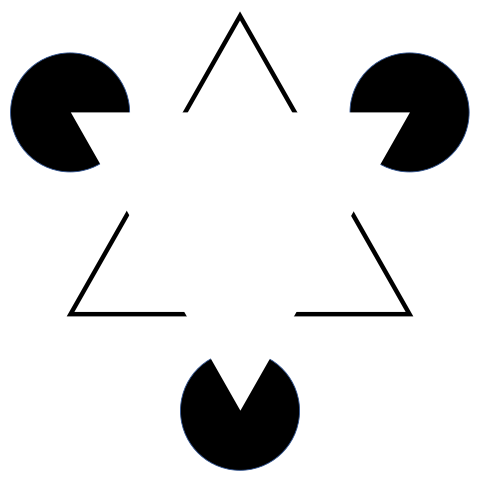
\includegraphics[width=0.45\textwidth]{triangle}
\centering
\caption{Jeden z możliwych wariantów trójkątu Kanzisy. Zeki określa ją jako przykład figury wątpliwie dwuznacznej.
Źródło: \url{https://upload.wikimedia.org/wikipedia/commons/thumb/5/55/Kanizsa_triangle.svg/480px-Kanizsa_triangle.svg.png}}

\end{figure}

W przypadku innych figur wieloznacznych, takich jak: \textit{sześcian Neckera} mózg nie może jednoznacznie ustalić rozmieszczenia krzyżujących się linii. Wszystkie one mogą leżeć na jednej płaszczyźnie lub część z~nich może znajdować się na pierwszym lub na drugim planie. Jest to przykład wieloznaczności prostej, która prawdopodobnie powstaje bez udziału wyższych ośrodków przetwarzania, ale jest wynikiem aktywności w pojedynczym obszarze neuroanatomicznym (por. rys. 1.5, (c)) \citep[s. 437-438]{Wieloznacznosc}. 


Tradycyjnym przykładem figur dwuznacznych są \textit{figury bistabilne} (por.rys. 1.5)
Jak sama nazwa wskazuje, potrafią one wytworzyć w mózgu dwa w pełni stabilne percepty, lecz świadomy wybór między nimi nie jest możliwy. (por. rys. 1.5, (a) i (b)) \citep[s. 92-93]{Zeki}.


Powstają one prawdopodobnie dzięki oddziaływaniom typu \textit{top-down}, czyli poprzez wpływ wyższych ośrodków przetwarzania na proces spostrzegania. Figura \textit{żona-teściowa} generuje dwie odrębne od siebie reprezentacje twarzy, co może sugerować to, że na proces interpretacji mogły mieć wpływ jakieś oddziaływania z innych obszarów mózgowych. Widać to  nawet dokładniej na przykładzie \textit{wazy Rubina}, gdzie dwa obrazy należą do różnych kategorii. Można przypuszczać, że w proces interpretacji wazy Rubina zaangażowane są na przemian dwa obszary mózgu: jeden odpowiedzialny za rozpoznawanie  twarzy, a drugi za rozpoznawanie obiektów użytkowych (por. rys. 1.5 (b)) \citep[s. 440-441]{Wieloznacznosc}.

Badania z zakresu neuroobrazowania wskazują, że moment przejścia od rozpoznania twarzy do rozpoznania wazy obejmuje zmianę aktywacji w rejonie zakrętu wrzecionowatego -- rejonu mózgu odpowiedzialnego za rozpoznawanie obiektów. Badania te wykazały również zaangażowanie kory czołowo-ciemieniowej przy zmianie perceptu z jednego na drugi. Interwencja wyższego obszaru mózgu odróżnia ten typ wieloznaczności od wieloznaczności prostej, która jest wynikiem wyłącznej aktywności w pojedynczym obszarze mózgu \citep[s. 441]{Wieloznacznosc}.

\begin{figure}[H]
    \centering
    \subfloat[figura bistabilna: żona-teściowa]{{
\includegraphics[width=4.5cm]{wife.png} }}%
    \qquad
    \subfloat[figura bistabilna: waza Rubina]{{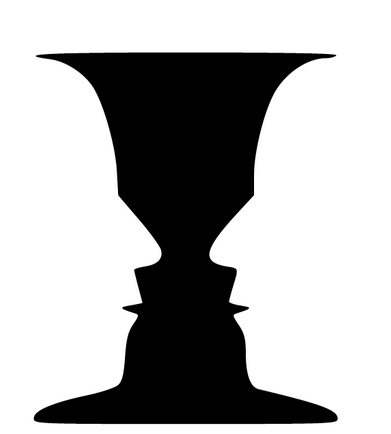
\includegraphics[width=4.5cm]{waza.png} }}%
    \qquad
    \subfloat[Sześcian Neckera] {{
\includegraphics[width=4.5cm]{necker.png} }}
    \caption{Za: (\citealt[s. 437, 440, 441]{Wieloznacznosc}).}
    
\end{figure}






Wieloznacznością wyższego rzędu nazywamy taką sytuację, kiedy to mózg spostrzega obraz tworzący pojedynczy stabilny percept, ale trudność stanowi interpretacja sytuacji, którą ten obraz przedstawia. Takimi obrazami są dzieła sztuki, zwłaszcza obrazy malarskie, kiedy to musimy wybrać jedną z wielu równorzędnych interpretacji. Dobrym przykładem może być obraz \textit{Dziewczyna z perłą,} znajdujący się w Królewskiej Galerii Malarstwa w Hadze. Samo dzieło przedstawia młodą kobietę z perłowym kolczykiem. Rolą odbiorcy jest wybranie odpowiedniej interpretacji wyrazu twarzy kobiety. Przykładowo, można ją uznać za zamyśloną, wystraszoną, a nawet emanującą erotyzmem. Możliwości interpretacyjne są szerokie i każda z nich ma równą wartość  i szanse na pojawienie się w świadomości odbiorcy dzieła  (por. rys. 1.6) \citep[s. 98-99]{Zeki}.

\begin{figure}[H]
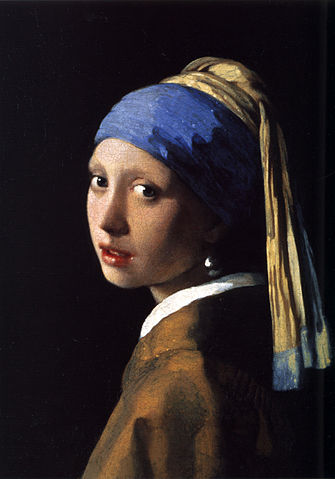
\includegraphics[width=6cm]{pearl}
\centering
\caption{Johannes Vermeer, Dziewczyna z perłą, około 1665r. Źródło: \url{https://en.wikipedia.org/wiki/Girl_with_a_Pearl_Earring}}
\end{figure}



\section{Teoria intencjonalnego opisu obrazu Romana Ingardena}

Jedną z ważniejszych fenomenologicznych prób zdefiniowania dzieła sztuki jest koncepcja intencjonalnego opisu dzieła malarskiego (obrazu) Romana Ingardena. Teoria ta opiera się na dwóch fundamentach: jednym z nich jest pojęcie intencjonalności, a  drugim rozróżnienie pomiędzy obrazem, a malowidłem \citep[s. 9]{Ingarden1958}.

Malowidło jest realną rzeczą wytworzoną na fizycznym materiale, takim jak: drzewo, płótno, szkło itp. Stanowi ono fizyczną podstawę bytu obrazu, która umożliwia jego zaistnienie w świecie \citep[s. 68]{Ingarden1958}. Istnienie malowidła jest warunkiem koniecznym istnienia obrazu, ale samo malowidło nie jest przedmiotem percepcji widza, służy jedynie jako nośnik treści, którą chce przekazać artysta przez obraz. Obraz powstaje w umyśle poprzez nadbudowanie nad malowidłem spostrzeżenia intencjonalnego\footnote{Intencjonalność jest rozumiana w fenomenologii jako świadomość czegoś. Świadomość jest jednocześnie ujmowaniem przedmiotu, myśleniem o nim oraz nadawaniem mu sensu \citep{sep-phenomenology}.}, które doprowadza odbiorcę do spostrzeżenia obrazu \citep[s. 70-73]{Ingarden1958}.

Rodzaj tego spostrzeżenia zależy od samej konstrukcji malowidła. Artysta poprzez umieszczenie na malowidle określonej kompozycji plam barwnych i kształtów może wpływać, świadomie lub nie, na rodzaj obrazu, który powstanie w umyśle odbiorcy dzieła. Obraz jest więc wytworem wyobraźni widza, a nie niezależnym przedmiotem istniejącym w świecie. Aby powstał obraz widz musi go wypełnić poprzez usunięcie występujących na malowidle \textit{miejsc niedookreślenia}. Poprzez takie dopełnienie dokonuje się \textit{konkretyzacja obrazu}, która stanowi bezpośredni przedmiot przeżycia estetycznego \citep[s. 99]{Ingarden1958}. Malowidło jest spostrzegane w prostym rzucie wzrokowym, ale interpretacja obrazu to złożony proces wymagający twórczej rekonstrukcji treści przedstawionej na malowidle \citep[s. 69]{Ingarden1958}






\section{Podsumowanie}

Semir Zeki sądzi, że głównym zadaniem mózgu wzrokowego jest zdobywanie wiedzy o świecie. Struktura kory wzrokowej umożliwia selekcję i interpretację informacji docierającej do oka. Mózg nieustannie porównuje nowe informacje z tymi, które już wcześniej zgromadził, dążąc do stworzenia stałej i stabilnej reprezentacji świata zewnętrznego. Zeki sugeruje, że artysta jest w jakimś sensie nieświadomym neuronaukowcem, badającym innymi środkami niż naukowcy możliwości mózgu. Percepcja sztuki wymaga od mózgu konfrontacji z wieloznacznością, która często występuje w sztuce \citep{Wieloznacznosc}.   Rozumienie sztuki przez Semira Zekiego odzwierciedla jego sposób rozumienia działania kory wzrokowej. Artysta wpływa na percepcje odbiorcy poprzez tworzoną sztukę zmuszając mózg do wyselekcjonowania istotnych informacji z docierającego sygnału w celu stworzenia przekonującej reprezentacji rzeczywistości \citep[s. 14-15]{Bremer}. Stworzenie stabilnej reprezentacji świata nie zawsze jest możliwe. Udowadniają to figury wieloznaczne, takie jak trójkąt Kanzisy. Figury tego typu stanowią przykład zmiennej lub niestabilnej reakcji mózgu na fizycznie niezmienny bodziec \citep[s. 73-74]{Zeki}.

W koncepcji Ramachandrana i Hirsteina rolą artysty jest nie tylko uchwycenie istoty obrazowanego przedmiotu, ale także wzmocnienie jego cech w taki sposób aby wywołać reakcję emocjonalną. Postulowana przez nich zasada przesunięcia szczytowego polega na wyolbrzymieniu pewnych charakterystycznych cech przedmiotu, które skutkuje silnym pobudzeniem układu limbicznego. Artysta stwarza w ten sposób bodziec wyolbrzymiony, który według  Ramachandrana i Hirsteina stanowi podstawę sztuki \citep[s. 332-336]{Rama}.

Przedstawione tutaj koncepcje bodźca wieloznacznego Semira Zekiego oraz bodźca wyolbrzymionego Ramachandrana i Hirsteina są jednymi  z pionierskich i bardziej oryginalnych prób  zdefiniowania dzieła sztuki w neuroestetyce. Obydwa podejścia zgodnie twierdzą, że sztuka zależy od funkcji kory wzrokowej, ale różni je sposób rozumienia tych funkcji. Koncepcja sztuki Zekiego dobrze wyjaśnia tylko niektóre rodzaje sztuki abstrakcyjnej i nowoczesnej. Obrazy kubistów są stworzone w taki sposób, że patrząc na obraz przedmiotu obserwujemy go z różnych perspektyw naraz, z których żadna nie jest wyeksponowana. Dlatego łatwo jest dopasować do dzieł kubistów pojęcie wieloznaczności w rozumieniu Zekiego, które z kolei nie pasuje zwykle do obrazów stworzonych w oparciu o tradycyjne techniki malarskie \citep[s. 16-17]{Bremer}. Z kolei potencjalną słabością postulowanej przez Ramachandrana i Hirsteina zasady przesunięcia szczytowego jest fakt, że pierwotnie została ona sformułowana na podstawie badań na zwierzętach. Ramachandran milcząco zakłada, że efekt przesunięcia szczytowego u zwierząt jest tożsamy z ludzkim przeżywaniem i rozumieniem sztuki \citep[s. 23]{Bremer}.

Interesującym rozszerzeniem koncepcji neuroestetycznych jest bardziej tradycyjne podejście fenomenologiczne. Fenomenologowie, tacy jak Roman Ingarden, nie starają się wyjaśnić sztuki poprzez zwracanie uwagi na aktywność w obrębie kory wzrokowej. Zamiast tego kładą oni nacisk na wzajemne interakcje twórcy dzieła z odbiorcą poprzez malowidło. Obraz jest u Ingardena nadbudowanym spostrzeżeniem intencjonalnym na fizycznym materiale, jakim jest malowidło. Percepcja obrazu zależy zarówno od cech fizycznego tworu na którym zostało ono zbudowane, ale także od indywidualnych przeżyć odbiorcy dzieła, który nadaje dziełu sens indywidualnie rekonstruując go w wyobraźni \citep[s. 68-70]{Ingarden1958}.


\chapter{Mechanizmy powstawania iluzji i ich wpływ na układ wzrokowy}

\section{Definicja bodźca iluzyjnego}

Mianem bodźca w psychologii określa się fizyczną formę energii zdolną zapoczątkować proces spostrzegania. Występują dwa rodzaje bodźców: bodźce \textit{dystalne} i \textit{proksymalne}. Bodziec dystalny to rodzaj bodźca, który pobudza układ percepcyjny odbiorcy na odległość przez emitowanie fal energii świetlnej lub energii fal dźwiękowych.  Bodziec proksymalny oddziałuje bezpośrednio na narządy zmysłów, pobudzając je. \citep[s. 23]{Hochberg1970}.


Jak już wspominano w rozdziale pierwszym, neuroestetyka traktuje dzieło sztuki jako bodziec specjalnego rodzaju, który wywiera znaczący wpływ na działanie systemu percepcyjnego osoby spostrzegającej obiekt będący dziełem sztuki. Percepcja takiego artystycznego bodźca wizualnego przypomina sytuację eksperymentalną, w której artysta pełni funkcję nieświadomego naukowca, a odbiorca sztuki jest osobą badaną, której reakcje są warunkowane obecnością bodźca, będącego w istocie dziełem sztuki \citep[s. 108]{neurostetyka}.
Typologia bodźców wizualnych zawiera te wspomniane już wcześniej, takie jak: bodziec wyolbrzymiony (\citeauthor{Rama}) i wieloznaczny (\citeauthor{Zeki}). W tym miejscu wymaga ona rozszerzenia o nową kategorię: \textit{bodziec iluzyjny}.


Według Piotra Przybysza bodziec iluzyjny jest takim obiektem, który  wywołuje w~umyśle odbiorcy wrażenie występowania cechy, przedmiotu lub relacji, które w rzeczywistości nie~występują. Iluzja jest więc zjawiskiem percepcyjnym, wytworem działalności mózgu \citep[s. 115]{neurostetyka}. Iluzje dotyczą wszystkich modalności zmysłowych wyróżnia się, m.in. \textit{wzrokowe, słuchowe} oraz \textit{dotykowe} \citep{Wyklad5}. Niniejsza praca koncentruje się na iluzjach wzrokowych.



\section{Typologia iluzji wzrokowych}

Istnieje kilka pomysłów na to jak można podzielić iluzje wzrokowe.  Typologia Jana Młodkowskiego wyróżnia na przykład  \textit{iluzje wzrokowe} -- związane tylko i wyłącznie z samym narządem wzroku oraz \textit{iluzje wizualne}, które powstają poprzez splot kilku różnych funkcji poznawczych \citep[s. 285]{Mlodkowski}. Iluzje wzrokowe mogą być jednoznaczne, czyli  stabilne jakościowo, to znaczy możliwe jest wygenerowanie tylko jednego perceptu lub złożone -- możliwa jest różna interpretacja jakościowa obrazu przez różne osoby w tym samym czasie lub przez jedną osobę, ale naprzemiennie (por. rys. 2.1) \citep[s. 287]{Mlodkowski}.


\begin{figure}[H]
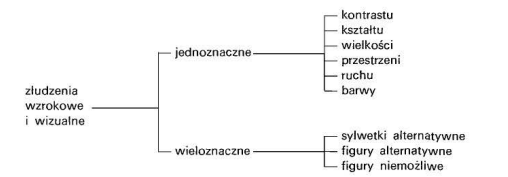
\includegraphics[width=\textwidth]{mlodkowski.png}
\caption{Typologia iluzji wzrokowych i wizualnych według Jana Młodkowskiego.}
\centering
\end{figure}

Przykładem iluzji kontrastu jest na przykład \textit{siatka Hermanna}. Siatka Hermanna jest złudzeniem optycznym odkrytym po raz pierwszy przez niemieckiego psychologa Ludimara Hermanna w 1870r. Spoglądając na figurę można dostrzec małe szare punkty na przecięciach białych linii, które znikają kiedy spojrzy się bezpośrednio na sam punkt przecięcia się tych linii. Występuje tutaj mocny kontrast pomiędzy białymi liniami a czarnym tłem, który tworzy wrażenie iluzji (por. rys. 2.2) \citep{Macperson}.

\begin{figure}[H]
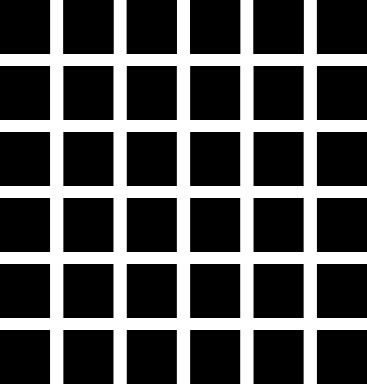
\includegraphics[width=0.3\textwidth]{grid.png}
\centering
\caption{ Na skrzyżowaniach białych pasów można dostrzec małe, szare kropki. Są one spowodowane zachodzeniem hamowania obocznego. Źródło: \url{https://upload.wikimedia.org/wikipedia/commons/0/0a/HermannGrid.gif}}
\end{figure}

 Iluzja siatki Hermanna jest wyjaśniania poprzez mechanizm działania pól odbiorczych i komórek zwojowych siatkówki oka. \textit{Polem odbiorczym (recepcyjnym)} w układzie wzrokowym nazywa się tę część pola widzenia,\footnote{Polem widzenia określa się fragment otoczenia, który można zobaczyć za jednym razem przez nieporuszające się oko \citep[s. 159]{Kalat}.} na którą reaguje dany neuron, pełniący funkcję receptora. Receptory te są połączone z komórkami dwubiegunowymi, które z kolei są przyłączone do komórek zwojowych siatkówki. Taki układ pozwala komórkom zwojowym pobierać informacje z pól recepcyjnych, należących do różnych receptorów jednocześnie \citep[s. 159]{Kalat}. Połączenia między neuronami mogą mieć charakter pobudzający i hamujący, więc pola recepcyjne także składają się z części hamującej i pobudzającej. Pobudzeniowa część pola recepcyjnego znajduje się w jego części centralnej, a hamująca w peryferyjnej. Neuron ulega pobudzeniu w chwili kiedy centrum jego pola recepcyjnego jest oświetlone \citep[s. 160]{Kalat}. Iluzja siatki Hermanna powstaje dzięki zjawisku \textit{hamowania obocznego}. Zjawisko to polega na osłabieniu aktywności neuronu przez aktywność neuronów sąsiadujących. Światło padające na powierzchnie siatkówki powoduje największe pobudzenie neuronów od wewnętrznej strony siatkówki (pobudzeniowa część pola recepcyjnego komórki zwojowej), a najsłabsze komórek nerwowych przylegających do zewnętrznej krawędzi obszaru naświetlania (hamująca część pola recepcyjnego komórki zwojowej). W ten sposób hamowanie oboczne wyostrza kontrast zachodzący pomiędzy obiektami będącymi w polu widzenia \citep[s. 161-162]{Kalat}.





Złudzenie Mullera-Lyera przedstawia figurę złożoną  z dwóch linii tej samej długości z  ostrzami zwróconymi do lub na zewnątrz drzewca. Złudzenie polega na tym, że linia z ostrzami zwróconymi na zewnątrz wydaje się dłuższa (por. rys. 2.3) \citep[s. 162-163]{Gregory}. Ze względu na kształt figurę tę nazywa się czasem złudzeniem strzały. Wyjaśnienie tego złudzenia przedstawia tzw. \textit{teoria perspektywy}. Stwierdza ona, że złudne figury, takie jak złudzenie strzały, sugerują głębie za pomocą perspektywy i, że owa sugestia głębi powoduje zmiany wielkości. Jest to możliwe, ponieważ figury złudne są w istocie płaskimi rzutami typowych trójwymiarowych przedmiotów. Jeśli zatem przedstawimy figurę złudną jako prosty rysunek perspektywiczny, czyli płaski rzut przestrzeni trójwymiarowej, to zauważymy, że te części figur,  które mogłyby przedstawiać przedmioty odległe, ulegają w naszej ocenie powiększeniu, te które przedstawiają przedmioty bliskie ulegają zmniejszaniu \citep[s. 171]{Gregory}. Istnieje proces spostrzeżeniowy zdolny do wywoływania tego typu zniekształceń: \textit{stałość oceny wielkości}. Jest to skłonność układu percepcyjnego do kompensowania zmian obrazu siatkówkowego zależnie od odległości postrzeganych obiektów (por. rys. 2.4) \citep[s. 175-176]{Gregory}.

\begin{figure}[H]
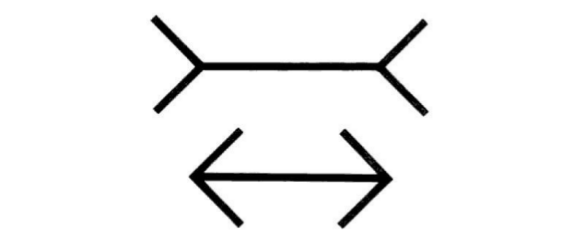
\includegraphics[width=0.7\textwidth]{muller.png}
\centering
\caption{Złudzenie Mullera-Lyera.}

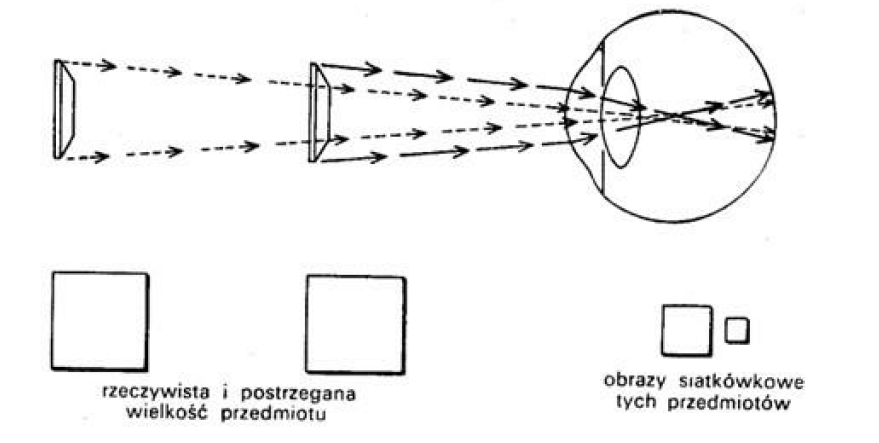
\includegraphics[width=0.7\textwidth]{stalosc.PNG}
\centering
\caption{Stałość oceny wielkości. Obraz przedmiotu zmniejsza o połowę swoje rozmiary przy każdym podwojeniu się odległości przedmiotu. Zmniejszanie się obrazu wraz z odległością przedmiotu stanowi podstawę większości złudzeń optycznych zniekształcających obraz przedmiotów. (Za: \citealt[s. 176]{Gregory}).}
\end{figure}

Złudzenie Ponzo przedstawia tor kolejowy zniekształcony przez perspektywę. Figura ta składa się z czterech linii, z których dwie położone są zbieżnie po bokach figury. Pomiędzy nimi umieszczono dwie równoległe linie jednakowej długości. Linia umieszczona w węższej części figury błędnie wydaje się dłuższa od tej położonej niżej (por. rys. 2.5) \citep[s. 163]{Gregory}. 

\begin{figure}[H]
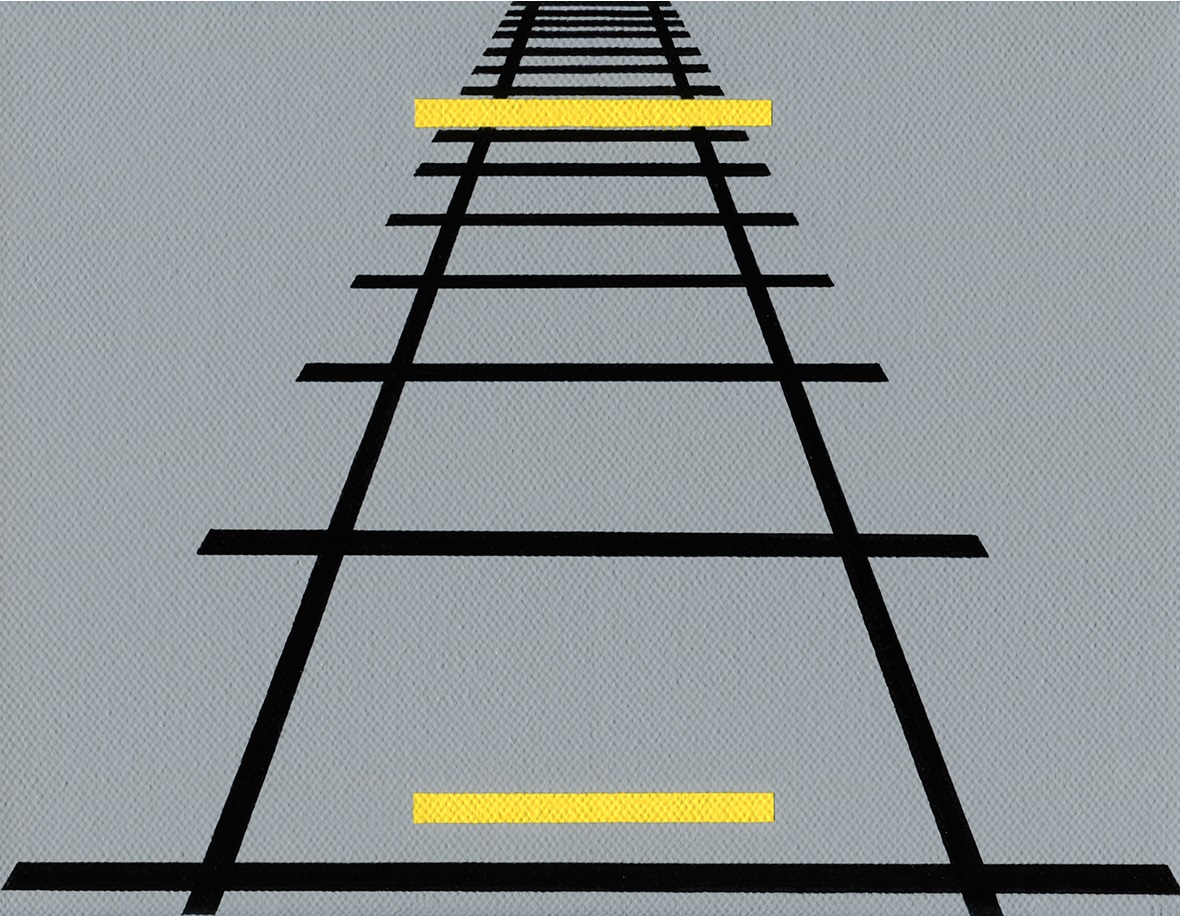
\includegraphics[width=0.5\textwidth]{ponzo.jpg}
\centering
\caption{Złudzenie Ponzo. Źródło: \url{https://www.illusionsindex.org/i/ponzo-illusion}}
\end{figure}

Wyjaśnieniem mechanizmu powstawania figury Ponza może być wspomniana wyżej stałość oceny wielkości, która działa analogicznie jak w przypadku złudzenia strzały, ale w literaturze przedmiotu można spotkać inne wyjaśnienia tego zjawiska. Gillam jest zdania, że wrażenie iluzji powoduje wykorzystanie \textit{skrótu perspektywicznego}, powszechnie stosowanego w malarstwie renesansowym \citep{Gillam1973}. Skrót perspektywiczny jest zabiegiem malarskim polegającym na zmniejszeniu postaci lub jej części na obrazie taki sposób, że wydaje nam się ona znacznie mniejsza niż jest w rzeczywistości. Zabieg ten stosuje się zwykle rysując obiekt od frontu, zgodnie z zasadami perspektywy linearnej (por. rys. 2.6) \citep[s. 382]{slownik}. 

\begin{figure}[H]
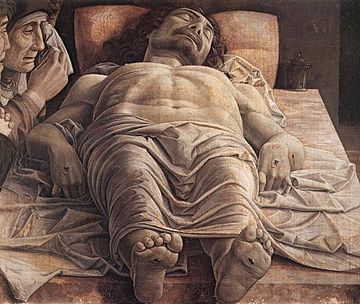
\includegraphics[width=0.5\textwidth]{chrystus.jpg}
\centering
\caption{Obraz Opłakiwanie zmarłego Chrystusa Andrea Mantegny. Postać Chrystusa została przedstawiona w skrócie perspektywicznym dlatego wydaje się pomniejszona. Źródło: \url{https://en.wikipedia.org/wiki/Lamentation_of_Christ_(Mantegna)}}
\end{figure}

Figury niemożliwe są przykładem figur, których rzeczywiste istnienie jest niemożliwe, a jedyną możliwą formą ich istnienia jest obraz. Są one przykładem wieloznacznych iluzji wzrokowych, ponieważ nie jest możliwe stworzenie jednego stabilnego perceptu podczas ich spostrzegania przez sprzeczność, która burzy każdą próbę ich jednoznacznej interpretacji.\footnote{Jest to cecha, która odróżnia je od opisywanych wcześniej \textit{figur bistabilnych}. W przypadku figur bistabilnych tworzą się dwa stabilne i tak samo wartościowe percepty, ale mózg ma problemy z wyborem jednego, dominującego w figurze. W figurach niemożliwych stworzenie chociaż jednego perceptu w całości jest niemożliwe \citep[s. 92-93]{Zeki}.} \citep[s. 290]{Mlodkowski}. Efekt iluzji w figurach niemożliwych dotyczy zawsze całości figury, a nie jej elementów składowych. Wynika to z bezpośrednio z mechanizmów percepcyjnych zachodzących w umyśle. Percepcja figury niemożliwej jest procesem złożonym, integrującym w całość wszystkie poprzedzające ją akty percepcji jednostkowej. Dopiero po zrekonstruowaniu w pamięci wszystkich elementów figury w całość i stworzeniu psychicznego odbicia rysunku w umyśle powstaje efekt iluzji \citep[s. 291]{Mlodkowski}. Figury niemożliwe stanowią zatem przykład \textit{iluzji top-down}, bo do ich interpretacji konieczna jest ingerencja wyższych obszarów przetwarzania informacji \citep[s. 4]{Wyklad5}. Tradycyjnym przykładem figury niemożliwej jest \textit{trójkąt Penrose'a} 



Trójkąt Penrose'a jawi się nam jako przedmiot skonstruowany z trzech równych belek w kształcie kwadratu złączonych ze sobą w taki sposób, że tworzą kąty proste, dając obraz przestrzennej trójwymiarowej figury. Żaden realnie istniejący obiekt nie może być zbudowany w podobny sposób. Trójkąt Penrose może występować jako dwuwymiarowa figura na płaszczyźnie płaskiej lub jako figura niemożliwa \citep[s. 291]{Mlodkowski}.

W belgijskim miasteczku Ophoven powstała rzeźba przypominająca trójkąt Penrose. Problem jego rzeczywistego odwzorowania jest następujący: rzeźba ta tworzy wrażenie iluzji tylko w momencie patrzenia na nią wprost. Przy spoglądaniu z innego miejsca wrażenie iluzji znika, a sama figura wygląda zupełnie inaczej (por. rys. 2.7) \citep[s. 29]{przybylski}. 

\begin{figure}[H]
     \centering
     \subfloat[][Przód figury]{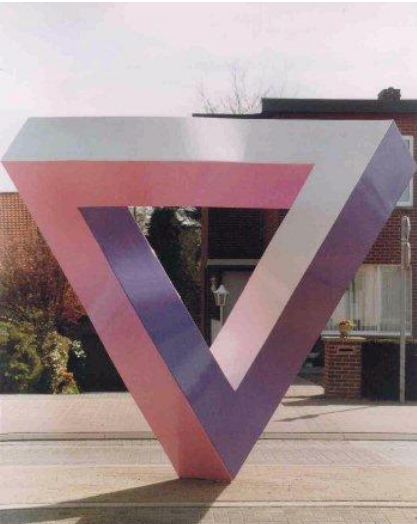
\includegraphics[width=0.45\textwidth]{penrose2.png}\label{Penrose2}}
     \qquad
     \subfloat[][Tył figury]{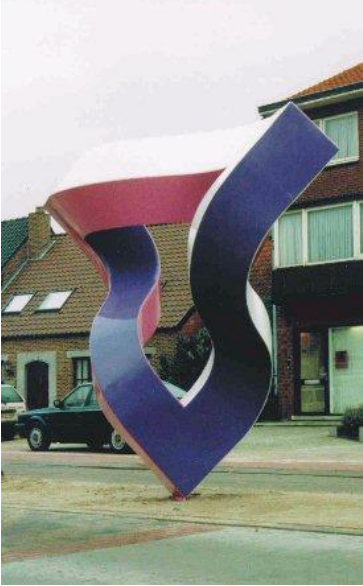
\includegraphics[width=0.35\textwidth]{penrose3.png}\label{Penrose3}}
     \caption{Trójkąt Penrose wybudowany w miasteczku Ophoven w Belgii (Za: \citealt[s. 29-30]{przybylski}).}
     
\end{figure}

Innym ciekawym przykładem figury niemożliwej są \textit{Schody Penrose'a}. jest to dwuwymiarowy obraz klatki schodowej umieszczonej na planie prostokąta. Schody zakręcają cztery razy pod kątem 90 stopni, biegnąc w górę i w dół, a przy tym tworząc ciągłą pętle. Dzięki temu można odnieść wrażenie, że wspinać się na nie można bez końca nigdy nie wchodząc na wyższe piętro (por. rys. 2.8) \citep[s. 71-78]{Bruno}.

\begin{figure}[H]
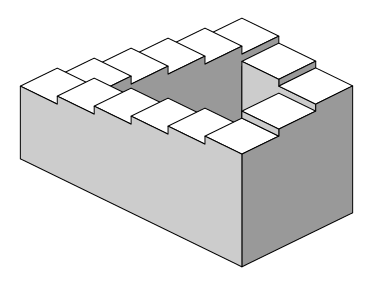
\includegraphics[width=0.5\textwidth]{schody.png}
\centering
\caption{Schody Penrose. Źródło: \url{https://upload.wikimedia.org/wikipedia/commons/thumb/3/34/Impossible_staircase.svg/372px-Impossible_staircase.svg.png}}
\end{figure}


Jedno z ciekawszych badań nad percepcją figur niemożliwych zostało przeprowadzone z użyciem fMRI. Zespół chińskich badaczy zbadał figurę niemożliwego trójzębu aby sprawdzić które obszary mózgu aktywują się podczas percepcji tego obiektu. W celu przeprowadzenia tego badania przygotowano dwa rodzaje bodźców: figurę możliwą w kształcie trójzębu (B) oraz podobną do niej figurę niemożliwą (A) (por. rys. 2.9, (a)) \citep[s. 19]{Wu2012}. Wyniki fMRI wskazały, że nie ma ośrodków mózgowych, które wykazują silniejszą odpowiedź w wariancie spostrzegania figury możliwej nad figurą niemożliwą. Jednakże zauważono także, że w percepcję figury niemożliwej zaangażowane są obszary: \textit{dolnego zakrętu skroniowego (ITG), zakrętu wrzecionowatego (FG)} oraz obszar \textit{prawego górnego zakrętu ciemieniowego (SPG)} (por. rys. 2.9, (b)). Prawy górny zakręt ciemniowy stanowi część strumienia grzbietowego w mózgu wzrokowym i odpowiada za widzenie przestrzenne. Natomiast zakręt wrzecionowaty oraz dolny zakręt skroniowy składają się na strumień brzuszny w mózgu wzrokowym, a ich aktywność może być związana z tworzeniem reprezentacji trójwymiarowych obiektów niemożliwych \citep[s. 20]{Wu2012}.

Badacze stwierdzają, że percepcja trójwymiarowych figur niemożliwych stanowi duże wyzwanie dla systemu percepcyjnego człowieka, a sam percept figury niemożliwej powstaje w wyniku próby złączenia ze sobą wielu rzutów perspektywicznych naraz, wynikających z trójwymiarowej struktury użytego bodźca \citep[s. 19-20]{Wu2012}.

\begin{figure}[H]
    \centering
    \subfloat[bodźce użyte w eksperymencie: A -- figura niemożliwa, B -- figura możliwa]{{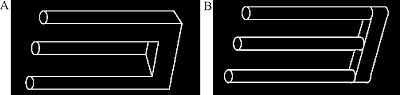
\includegraphics[width=\textwidth]{impossible_possible.jpg}}}%
    \qquad
    \subfloat[Obszary mózgu różniące się aktywnością w warunku percepcji figury możliwej oraz niemożliwej (poziom istotności: p < 0.05).]{{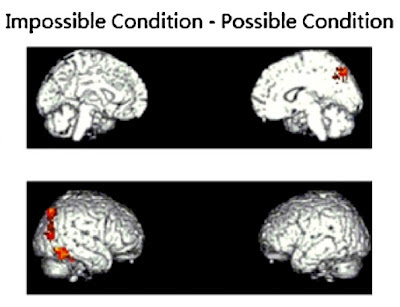
\includegraphics[width=\textwidth]{regiony.jpg} }}%
    \caption{}
    \end{figure}
    \clearpage
    
\section{Dwa szlaki przetwarzania informacji wzrokowej w mózgu} 

Amerykańska neurofizjolog Margaret Livingstone, stworzyła koncepcję starającą się wyjaśnić powstawanie iluzji ruchu występującej podczas oglądania niektórych dzieł impresjonistów. Wyodrębniła ona dwa równoległe szlaki przetwarzania informacji w mózgu wzrokowym. Ewolucyjnie starszy szlak służący analizie poziomu luminancji na obrazie, rozumianej jako ilość światła odbitego od powierzchni i odebranego przez narząd wzroku oraz ewolucyjnie młodszy, występujący u naczelnych, szlak służący analizie barwy, który jest niewrażliwy na zmiany ilości światła. Szlak wzrokowy odpowiedzialny za analizę światła jest nazywany czasem szlakiem \textit{Gdzie}, a szlak wzrokowy odpowiadający barwie nazywa się szlakiem \textit{Co}. Zawartość każdego obrazu jaki spostrzegamy jest według tej koncepcji analizowana niezależnie przez dwa różne systemy wzrokowe \citep[s. 51]{livingstone2002}.
Każdy z wyżej wymienionych szlaków przetwarzania wzrokowego jest inicjowany przez inny typ komórek zwojowych siatkówki oka. Szlak \textit{Co} przebiega pomiędzy pierwszorzędową korą wzrokową, a korą skroniową, a jego działanie jest inicjowane przez specjalny typ komórek P zwane także komórkami \textit{parvo}\footnote{Parvus, parvum, parvo(łac.) -- mały, niewielki.}. Specjalizuje się on w analizie barwy, kształtu oraz percepcji twarzy. Szlak \textit{Gdzie} przebiega od górnej części płata potylicznego do kory ciemieniowej. Tworzą go komórki typu M -- magno\footnote{Magnus, magna, magno(łac.) -- duży, ogromny.}, a sam szlak przejawia wysoką wrażliwość na kontrast, ruch, jest szczególnie wyczulony na identyfikację obiektów w przestrzeni \citep[s. 740-741]{Livingstone1988}. Każdy z opisanych tutaj szlaków przetwarzania -- \textit{parvo} i \textit{magno} jest zaangażowany na innym szczeblu przetwarzania wzrokowego. Szlak \textit{parvo} zajmować się będzie szczegółową analizą obrazu, a szlak \textit{magno} będzie zajmował się odtworzeniem rozmieszczenia obiektów w przestrzeni (por. tabela 2.1 i rys. 2.10) \citep[s. 51]{livingstone2002}.
\begin{table}[H]
\centering
\begin{tabular}{@{}|c|c|c|@{}}
\toprule
Wrażliwość na & System "Gdzie?" & System "Co?" \\ \midrule
Kolor & Niewrażliwy na kolory & Niesie informacje o kolorze \\ \midrule
Kontrast & Wysoka wrażliwość na kontrast & Niska wrażliwość na kontrast \\ \midrule
\begin{tabular}[c]{@{}c@{}}Szybkość \\ przetwarzania\\ danych\end{tabular} & Szybszy & Wolniejszy \\ \midrule
\begin{tabular}[c]{@{}c@{}}Rozdzielczość\\ obrazu\end{tabular} & Mniejsza & Większa \\ \bottomrule
\end{tabular}
\caption{Tabela prezentująca działanie szlaku Gdzie? i szlaku Co? w mózgu wzrokowym (Za: \citealt[s. 51]{livingstone2002})}
\end{table}


Claude Monet podczas malowania swojego słynnego obrazu \textit{Impresja. Wschód Słońca}, zastosował ciekawą sztuczkę. Wszystkie obiekty na obrazie posiadają taki sam poziom luminancji, różnią się jedynie kolorystyką. Dla pierwszego strumienia obraz ten jawi się cały w odcieniach szarości, a słońce jest na nim prawie niewidoczne. Dla drugiego, poświęconego analizie koloru, słońce jest wyraźnie widoczne. Do mózgu docierają  sprzeczne informacje jednocześnie z dwóch różnych strumieni przetwarzania. Sprzeczność ta jest powodem tworzenia się iluzji ruchu (por. rys. 3.14) \citep[s. 116]{neurostetyka}.
 
\begin{figure}[H]
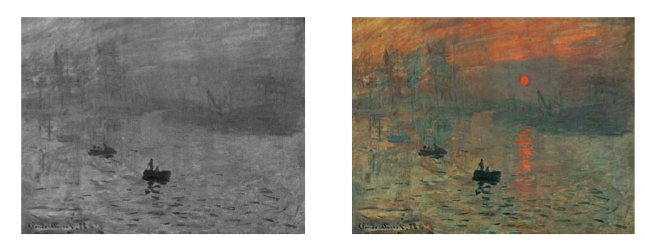
\includegraphics[width=\textwidth]{monet.png}
\centering
\caption{W oryginalnej wersji (po prawej) słońce i jego odbicie są wyraźnie widoczne. Po nałożeniu filtru szarości wrażenie ustępuje -- widzimy teraz, że cały obraz charakteryzuje się podobnym poziomem luminancji (Za: \citealt[s. 116]{neurostetyka}).}
\end{figure}



\section{Iluzja głębi}

Życie codzienne człowieka odbywa się w przestrzeni wyznaczonej przez trzy wymiary: \textit{horyzontalny} (w prawo lub lewo), \textit{wertykalny} (góra lub dół), \textit{w głąb} (z przodu lub z tyłu) \citep[s. 221]{Francuz}.
Jeśli posiadamy sprawny system wzrokowy to w tak rozumianej przestrzeni potrafimy się bez problemu odnaleźć. Oczywiście nie zawsze jest to proste, a sprawność poruszania się w przestrzeni trójwymiarowej zależy także od stopnia wyćwiczenia w postrzeganiu trójwymiarowości oraz od naszego umiejscowienia względem percypowanego obiektu. Łatwiej jest doświadczyć głębi obserwatorowi umieszczonemu w pozycji centralnej, na wprost względem obiektu \citep[s. 223]{Francuz}. Wymiar horyzontalny i wertykalny wyznaczają płaszczyznę prostopadłą do osi widzenia, a wymiar w głąb wyznacza linię równoległa do niej \citep[s.221-222]{Francuz}. Widzenie sceny w trzech wymiarach jest procesem polegającym na  widzeniu zbioru płaszczyzn prostopadłych do osi widzenia, które umieszczone są  w różnej odległości od obserwatora, w taki sposób żeby umieścić je dodatkowo na osiach wzdłuż trzeciego wymiaru. Nie widzimy w scenie tych rzeczy, których izometryczne rzuty na płaszczyznę prostopadłą do osi widzenia przyjmują wartości zerowe na którymkolwiek z pozostałych wymiarów \citep[s. 220-221]{Francuz}.

Mechanizmem umożliwiającym ludziom zdolność widzenia głębi jest \textit{widzenie stereoskopowe}. Zdolność do tego typu widzenia powstała jako odpowiedź na wyzwania środowiska w toku ewolucji. Jest to umiejętność służąca przede wszystkim przeżyciu w stale zmieniającym się środowisku. W naturalnych warunkach system wzrokowy jest w stanie objąć uwagą obszar do około 6 metrów wokół nas. Organizm posiadający zdolność widzenia stereoskopowego jest w stanie bardzo szybko zareagować na intruza przekraczającego tę prywatną przestrzeń i dzięki temu zachować życie \citep[s. 221]{Francuz}. Dwa najważniejsze elementy umożliwiające widzenie stereoskopowe to \textit{rozbieżność dwuoczna} i tzw. odruchy wergencyjne: \textit{dywergencja} i \textit{konwergencja} \citep[s. 223]{Francuz}. Doświadczenie głębi widzenia powstaje dzięki integracji dwuwymiarowych obrazów padających na komórki siatkówki oka. Integracja ta odbywa się na korowych etapach szlaku wzrokowego.\footnote{ Wstępna interpretacja sygnału dotyczącego rozbieżności dwuocznej odbywa się  w korze V1. Dalsze etapy tego przetwarzania prowadzone są w strukturach płatów ciemieniowych a zwłaszcza w obszarze V5 \citep[s. 221]{Francuz}.} Wynikiem integracji jest obraz zawierający informacje o uporządkowaniu widzianych płaszczyzn w głąb \citep[s. 222-223]{Francuz}. Rolą odruchów wergencyjnych jest sterowanie ułożeniem gałek ocznych, w taki sposób żeby umożliwić jak najlepsze kadrowanie sceny wizualnej. Konwergencyjny ruch oczu występuje jako przejaw większego zainteresowania obiektami położonymi bliżej obserwatora, natomiast ruch dywergencyjny wskazuje na zainteresowanie obiektami położonymi dalej od obserwatora, ale do granicy sześciu metrów, która stanowi kres zasięgu widzenia przestrzennego \citep[s. 223]{Francuz}.

Pozostaje zatem pytanie w jaki sposób można celowo wywołać wrażenie głębi na płaskim obrazie? Jedną z możliwych odpowiedzi jest koncepcja wskaźników głębi postulowana m.in. przez Bronisława Deręgowskiego. Deręgowski twierdzi, że trójwymiarowość na obrazie można pokazać na dwa sposoby. Pierwszy z nich pozwala uwypuklić w przedmiocie trójwymiarowym te cechy, które pozwalają łatwo odróżnić go od otoczenia. Taki obiekt nazywa się wtedy \textit{obiektem epitomicznym} \citep[s. 20]{Deregowski}. Można też zaprezentować przedmiot w taki sposób żeby ukazywać wyłącznie jego cechy trójwymiarowe. Jest to wtedy \textit{obiekt eidoliczny} \citep[s. 21]{Deregowski}. W pierwszym przypadku ukazany przedmiot tworzy \textit{efekt epitomiczny}. Występuje on wtedy kiedy zawarta w obrazie liczba informacji, wystarcza do wywołania obrazu percepcyjnego przedstawianego przedmiotu, bez bezpośredniego przywołania jego trójwymiarowości. Efekt eidoliczny otrzymywany jest dzięki użyciu przez artystę specjalnych \textit{wskaźników głębi}. Wskaźniki które będą poniżej omawiane nazywa się jednoocznymi ponieważ stosuje się je w celu wywołania iluzji głębi na płaskim obrazie. Zabieg ten udaje się osiągnąć bez wzajemnej współpracy obu gałek ocznych \citep[s. 19-20]{Deregowski}.

Jednooczne wskaźniki głębi stanowią podstawę rozumienia relacji przestrzennych na płaskim obrazie. Trafność rozumienia tych wskaźników jest wynikiem uczenia się w jaki sposób określone wzorce płaszczyzn, konturów i barw odnoszą się do rzeczywistego występowania tych obiektów w świecie rzeczywistym \citep[s. 223]{Francuz}. Hipotezę mówiącą o tym, że rozumienie relacji przestrzennych jest wynikiem procesu uczenia wspierają wyniki badań międzykulturowych. W jednym z nich Robert Serpell i Jan B. Deręgowski udowodnili, że wprowadzenie do sceny polowania jednoocznych wskaźników głębi, których rozumienie jest oczywiste dla osób pochodzących z kręgu kultury zachodniej, takich jak  wskaźnik linii horyzontu,  zbieżności krawędzi czy właściwego stopniowania wielkości obiektów znajdujących się na pierwszym i drugim planie obrazu nie wystarcza do wywołania wrażenia iluzji głębi. Mieszkańcy Ghany, Zambii czy Ugandy niezmiennie interpretowali niżej przedstawioną scenę jako polowanie na słonia, a nie na Antylopę (por. rys. 2.11) \citep{Serpell}.

\begin{figure}[H]
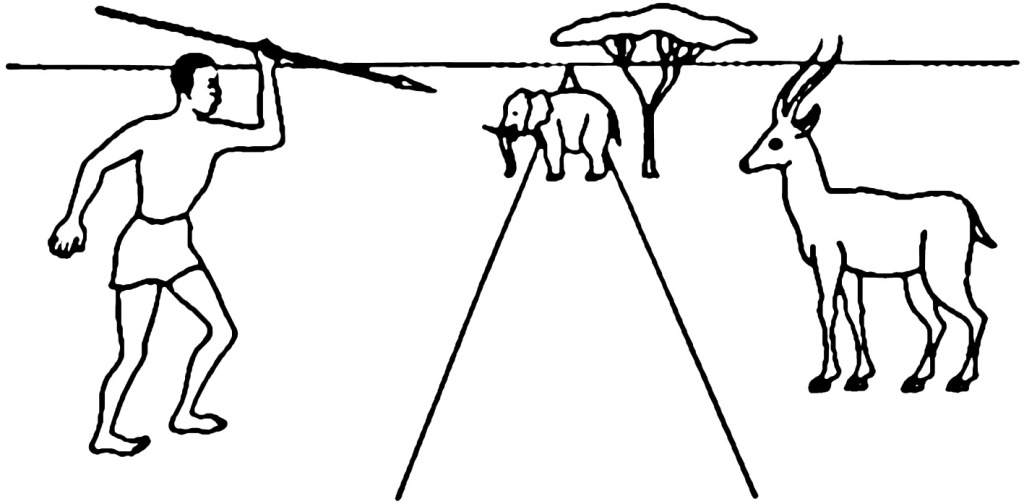
\includegraphics[width=0.7\textwidth]{Hudson.jpg}
\centering
\caption{Ilustracja z testu percepcji głębi W. Hudsona używanego w badaniu Roberta Serpella i  Jana B. Deręgowskiego (\citeyear{Serpell})  (Za: \citealt{Hudson}).}
\end{figure}


\section{Podsumowanie}

Literatura na temat mechanizmów powstawania i typów iluzji wzrokowych jest bardzo szeroka. Rozdział ten siłą rzeczy przedstawia tylko wybrane koncepcje, które zdaniem autora najlepiej tłumaczą powstawanie złudzeń. Złudzenia optyczne są szeroko wykorzystywane w malarstwie jako środek artystycznego wyrazu. Zgodnie z postulatami neuroestetyków niejednoznaczność obrazu może być silnie przyciągać uwagę i odpowiadać za powstawanie wrażeń estetycznych. Dlatego też malarze coraz częściej wykorzystują iluzje w swoich pracach. Nurtem sztuki, który w całości koncentruje się na zwodzeniu aparatu percepcyjnego odbiorcy jest \textit{sztuka optyczna (op-art)}.








\chapter{Neuroestetyczna analiza iluzji wzrokowych na przykładzie dzieł Eschera}
\section{Wstęp}



 Większość dzieł powstających w ramach nurtu sztuki optycznej (op-art) składa się z powtarzających się geometrycznych wzorów. Charakterystyczną cechą o1p-artu jest zdolność do wywoływania iluzorycznych obrazów i sensacji wzrokowych u odbiorcy na skutek eksploatacji właściwości fizycznych oka i mechanizmów działania samego mózgu. Cechą którą odróżnia op-art od malarstwa iluzjonistycznego jest to, że iluzjonizm wykorzystuje umiejętność widza do dopełnienia brakującej części widzianego dzieła w umyśle i w efekcie tejże rekonstrukcji powstaje finalnie wrażenie iluzji. Natomiast w op-arcie iluzja powstaje jako efekt poddawania w wątpliwość normalnych procesów procesów widzenia, głównie przez specyficzne optyczne oddziaływanie danego dzieła na odbiorcę \citep[s. 353-354]{Reichard}. Jednym z pierwszych twórców tworzących w tym nurcie był Węgier Victor Vasarely (1908-1997). Uważany jest on za jednego z prekursorów  nurtu sztuki optycznej. Swoje pierwsze eksperymenty rozpoczął już w latach 30 XX. wieku. Charakterystyczne dla niego jest wykorzystanie figur w taki sposób, żeby wykazać dwuznaczność i zwodniczość zjawisk optycznych poprzez wykorzystanie nieregularnych geometrycznych układów \citep[s. 356-358]{Reichard}.
 
 
Jednym z artystów tworzących w nurcie op-artu jest Maurits Cornelis Escher (1898 - 1927) -- holenderski malarz i grafik. Escher zasłynął z tego, że w swoich pracach ukazywał formy przestrzenne sprzeczne z doświadczeniem wzrokowym. Analiza obrazów Eschera zostanie przeprowadzona w oparciu o \textit{trójpoziomowy semiotyczny model dzieła sztuki malarskiej Moniki Bianki Florek}.


\section{Trójpoziomowy semiotyczny model dzieła sztuki malarskiej}

Monika Bianka Florek proponuje trójpoziomowy model budowy dzieła malarskiego. Model ten został zainspirowany koncepcją języków symbolicznych Nelsona Goodmana. Zdaniem Goodmana malarstwo, muzyka, rzeźba są przykładami odmiennych gatunków sztuki, które powstają w wyniku zastosowania podobnych procedur światotwórczych opartych o określony alfabet symboli malarskich \citep[s. 388]{Florek2006}.

Według proponowanego przez Florek ujęcia w dziele malarskim można wyróżnić:
\begin{itemize}
    \item poziom inskrypcji,
    \item poziom etykiet,
    \item poziom światowości (za: \citealt[s. 388]{Florek2006}).
\end{itemize}


 Na poziomie \textit{inskrypcji} występują \textit{inskrypcje atomiczne}, czyli plamy barwne oraz wszystkie inne inskrypcje -- kształty, linie -- wchodzące w skład \textit{inskrypcji złożonych}. Zdaniem Goodmana inskrypcje tworzą materialną bazę dzieła, ponieważ stanowią alfabet symboliczny języka malarskiego, czyli uporządkowaną strukturę, którą można opisać na podobieństwo struktur syntaktycznych w językach werbalnych. Warstwa inskrypcji jako warstwa niesymboliczna pozostaje często przez widza niezauważona, ale jest bardzo istotna, ponieważ to od niej zależy jakie znaczenie symboliczne posiada obraz. Specyfiką języka barw jest to, że trudno jest przeprowadzić w nim kategorialną klasyfikację takich inskrypcji. Wynika to z faktu nazwanego przez Goodmana \textit{gęstością}. Gęstość sprawia, że nie jest możliwe dokonanie rozłącznej kategoryzacji barw. Oko widza jest zdolne uchwycić różnice barwne tylko wtedy, jeśli trzy barwy lub więcej są złączone razem, a różnice kontrastowe między nimi są wyraźnie zaznaczone \citep[s. 389]{Florek2006}.
 
Inskrypcje złożone różnią się między sobą komplikacją złożeń. Przy czym owa komplikacja nie musi być skorelowana ze złożonością obiektu do którego inskrypcja się odnosi. Bardzo prosta inskrypcja złożona jaką jest koło, może być symbolem bardzo skomplikowanego obiektu, jakim jest kobieta. Posługiwanie się inskrypcjami o określonym poziomie złożenia często jest wskaźnikiem stylu, w jakim został wykonany obraz \citep[s. 390]{Florek2006}.

Podobnie jak nie wszystkie litery alfabetu tworzą sensowne wyrazy, tak nie każda konfiguracja plam barwnych tworzy inskrypcję złożoną. Sposób w jaki określone plamy barwne zostaną zinterpretowane zależy od tego jakie reguły składania zastosują artyści. Wspomniane w poprzednim rozdziale wskaźniki głębi (por. np. \citealt[s. 25]{Deregowski} oraz \citealt[s. 53]{Hochberg1970}) wykorzystywane są często aby stworzyć iluzję głębi na płaszczyźnie dwuwymiarowej. Przez wykorzystanie tych wskaźników można oszukać umysł, że ma do czynienia z głębią \citep[s. 391]{Florek2006}

Prześledźmy w jakich sposób Escher korzysta ze wskaźników głębi w swoich pracach.
Obrazy Eschera wykorzystują często \textit{wskaźnik perspektywy liniowej}. Na obrazie \textit{Galeria} można dostrzec jeden punkt zbieżności umieszczony na końcu linii horyzontu, będącej także na wysokości oczu. Zastosowanie skrótu perspektywicznego z jednym punktem zbieżności umieszczonym frontalnie w przestrzeni sprawia wrażenie, że korytarz galerii jest mniejszy niż w rzeczywistości. Działa tutaj  prawo stałości oceny wielkości, zgodnie z którym subiektywnie postrzegamy przedmioty leżące w różnej odległości od obserwatora jako takie same, mimo iż na siatkówce oka przedmioty leżące dalej są mniejsze (por. rys. 3.1 (a)) \citep[s. 32-33]{Deregowski}.\textit{Wieża Babel} posiada aż trzy punkty zbiegu. Linie poziome zbiegają się w parę znikających punktów na horyzoncie. Ponieważ linia horyzontu jest umieszczona bardzo wysoko wydaje się nam, że scena jest oglądana z dużej wysokości.  Pionowe linie zbiegają w dół do nadiru potęgując wrażenie dużej wysokości (por. rys. 3.1 (c) oraz rys. 3.2) \citep{EscherMath2006}. Na litografii \textit{Balkon} Escher używa perspektywy aby wywołać wrażenie trójwymiarowości na płaskim obrazie. Patrząc na ten obraz wydaje się nam, że spoglądamy na trójwymiarowy obiekt, a nie na płaską powierzchnie (por. rys. 3.1 (b)) \citep{EscherMath2006}.

\begin{figure}[H]
    \centering
    \subfloat[Galleria (1946)]{{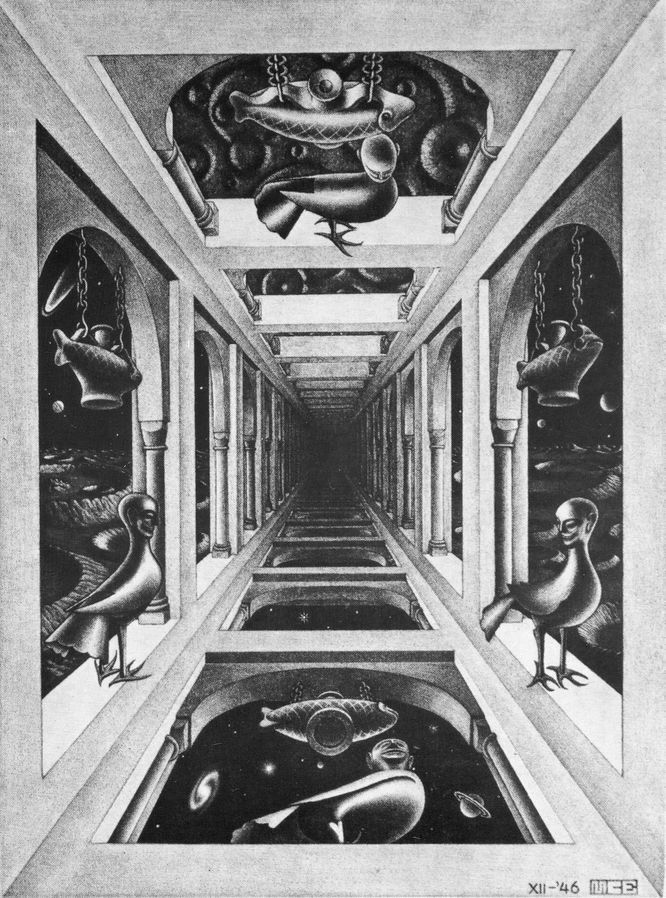
\includegraphics[width=8cm]{gallery.jpg}}}%
    \qquad
    \subfloat[Balkon (1945)]{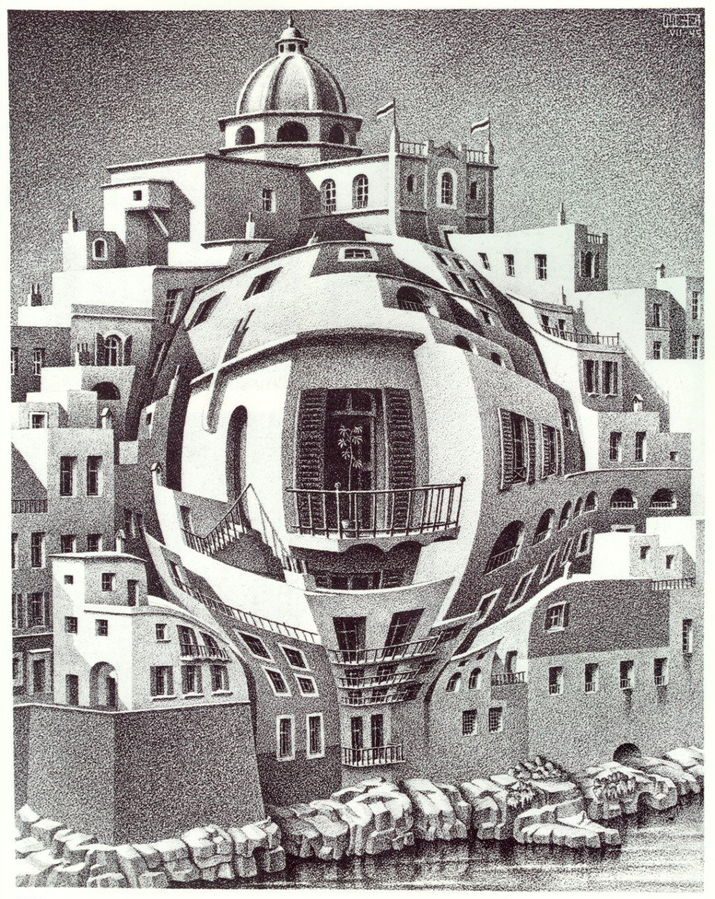
\includegraphics[width=7cm]{Balcony.jpg}}
    \qquad
    \subfloat[Wieża Babel (1928)]{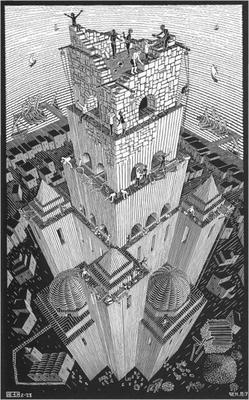
\includegraphics[width=6cm]{babel.jpg}}
    \caption{Źródło: \url{www.mcescher.com} [Dostęp: 14.06.19]}
    \end{figure}
    \clearpage
    
\begin{figure}[H]
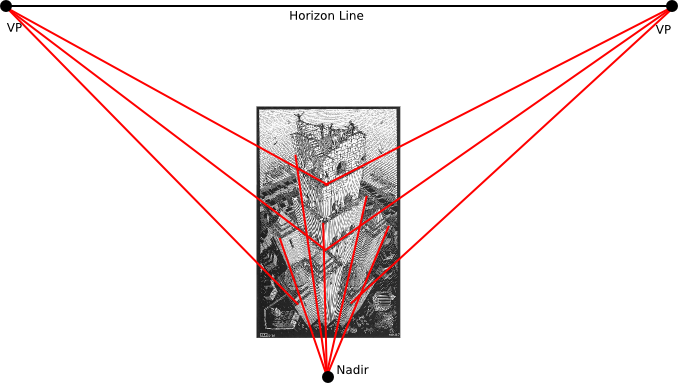
\includegraphics[width=\textwidth]{babelvps.png}
\centering
\caption{Punkty zbieżności na obrazie Wieża Babel (1928)  (Za: \citealt{EscherMath2006}).}
\end{figure}



Drugi poziom dzieła sztuki: \textit{poziom etykiet}, charakteryzuje się obecnością nadbudowanych nad inskrypcjami \textit{etykiet}, które niosą ze sobą kontekst myślowy lub wyobrażeniowy. Przykładowo, jeśli na poziomie pierwszym natykamy się na inskrypcje złożoną o kształcie czerwonej plamy, to na poziomie drugim zidentyfikowana jest ona jako czerwona piłka, pomidor lub głowa w czepku \citep[s. 391]{Florek2006}.

Każda etykieta jest związana z określoną inskrypcją malarską, jednak nie jest to wcale warunek konieczny, np. z inskrypcją czerwonej plamy może być związane wiele etykiet, jak czerwona piłka, boja, pojemnik, itd. Mówiąc potocznie każda inskrypcja może być odczytywana na wiele różnych sposobów. Ta wielość odczytań jest często wykorzystywana w obrazach abstrakcyjnych \citep[s. 392]{Florek2006}.
Spójrzmy na obraz \textit{Ulica Scanno w Abruzji}. Obecnym na obrazie inskrypcjom złożonym możemy nadać etykiety takie jak: "dom", "ulica", schody i inne. Przejście na poziom etykiet sprawia, że znak malarski rozpatrywany dotąd bez żadnego odniesienia do przedmiotu realnego staje się jego symbolem (por. rys. 3.3) \citep[s. 392]{Florek2006}.

    
\begin{figure}[H]
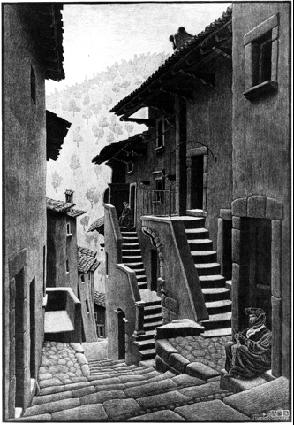
\includegraphics[width=0.6\textwidth]{street.jpg}
\centering
\caption{Ulica w Scanno w Abruzji (1930) Źródło: \url{www.mcescher.com} [Dostęp: 14.06.19]}
\end{figure}

Z kolei na trzeci poziom: \textit{poziom światowości} składają się zrealizowane na obrazie sytuacje symboliczne wraz z nadbudowanymi nad nimi możliwymi odniesieniami rekonstruowanymi w procesie odbioru dzieła. Razem zestawione tworzą świat przedstawiony w dziele malarskim. Według Goodmana każde dzieło sztuki powstaje z elementów jakiegoś innego świata (np. świata rzeczywistego) za pomocą światotwórczych procesów składania, takich jak: rozkładanie, porządkowanie , usuwanie, dodawanie i wreszcie deformowanie świata wyjściowego. Operacje te mogą zachodzić na różnych poziomach dzieła sztuki, a między każdym ze stworzonych światów, zdaniem Goodmana, zachodzą relacje typu referencyjnego, dzięki którym obrazy mogą wzajemnie odnosić się do siebie \citep[s. 394- 395]{Florek2006}. Na rysunku 3.3 sytuację symboliczną tworzy widok ciasnej uliczki otoczonej po obu stronach przez domostwa zbudowane w typowo włoskim stylu architektonicznym. Zbudowana w ten sposób scena symboliczna tworzy odrębny świat do którego odsyła dzieło sztuki \citep[s. 395]{Florek2006}.

 \section{Różnice pomiędzy percepcją, a interpretacją dzieła malarskiego}
 
Dyskusja na temat różnicy między interpretacją, a percepcją dzieła sztuki rozpatrywana jest przez przyzmat \textit{idealnego perceptora} i \textit{idealnego interpretatora} sztuki.

Idealny perceptor reprezentuje i maksymalizuje to co w standardowym znaczeniu nazywane jest naturalistycznym podejściem do sztuki. Istotą naturalistycznego podejścia jest traktowanie odbioru dzieła sztuki jako procesu rządzonego przez prawa percepcji i reakcji emocjonalnej. Estetyka obrazu jest w takim wypadku konsekwencją wykorzystania przez artystę reguł rządzących percepcją i wzbudzaniem emocji, którym podlega obraz \citep[s. 396]{Florek2006}.

Z pojęciem idealnego interpretatora łączy się natomiast spojrzenie na widza jako współkreatora dzieła sztuki, a samo dzieło traktuje się jako symbol wymagający czynnej interpretacji ze strony podmiotu. Rolą odbiorcy jest odkodowanie treści zawartej przez artystę. Bierna postawa preceptora wobec dzieła sztuki zostaje zastąpiona przez czynną postawę interpretatora  \citep[s. 396]{Florek2006}.

W przypadku sztuki iluzyjnej obecne są jedynie inskrypcje malarskie, które działają pobudzająco na układ percepcyjny odbiorcy \citep[s. 397]{Florek2006}. Dzieło sztuki stanowi tutaj wzmocniony bodziec odpowiedzialny za powstawanie wrażeń estetycznych (por. \citealt[s. 353]{Rama}.) Aby wywołać reakcję artysta ma do dyspozycji farby malarskie, prawa percepcji i świadomość (przeczucie), że manipulowanie nimi pozwoli osiągnąć zamierzony efekt artystyczny \citep[s. 396 - 397]{Florek2006}.








\section{Figury niemożliwe na obrazach Eschera}

Escher w swojej twórczości często wykorzystuje figury niemożliwe. Na litografii \textit{Belweder} możemy dostrzec budowlę w całości skonstruowaną z figur niemożliwych (por. rys. 4.3) \citep[s. 142]{Locher}.



\textit{Belweder} ukazuje budowlę, która nie mogłaby istnieć w świecie rzeczywistym, ponieważ narusza wszystkie znane prawa geometrii euklidesowej. Na przykład, filary budynku są tak rozmieszczone, że występują zarówno w górnej części frontowej budynku, jak i w dolnej, tylnej części budynku, a mimo tego nie odchylają się nawet o kilka stopni, sprawiając wrażenie idealnie pionowych kolumn. Co więcej, drabina widoczna na obrazie w swej dolnej, początkowej części  wydaje się pochylać bardziej do wnętrza budynku, a im bardziej ona pnie się w górę, tym bardziej wychyla się na zewnątrz. W dolnym fragmencie rysunku widzimy także człowieka trzymającego w dłoniach \textit{sześcian Neckera} (por. rys. 3.4).

\begin{figure}[H]
    \centering
    \subfloat[Belweder (1958)]{{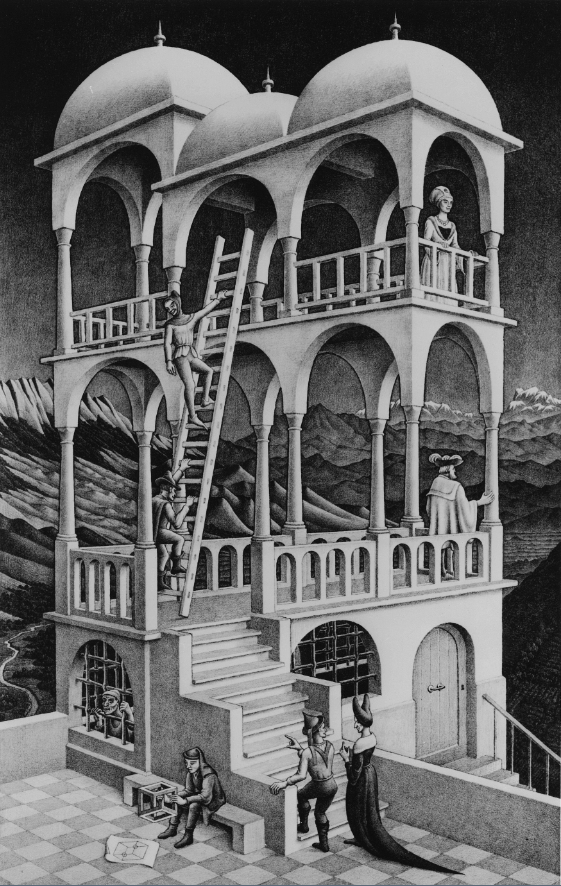
\includegraphics[width=8cm]{Belweder.png}}}%
    \qquad
    \subfloat[Fragment obrazu Belweder. Mężczyzna trzymający sześcian Neckera.]{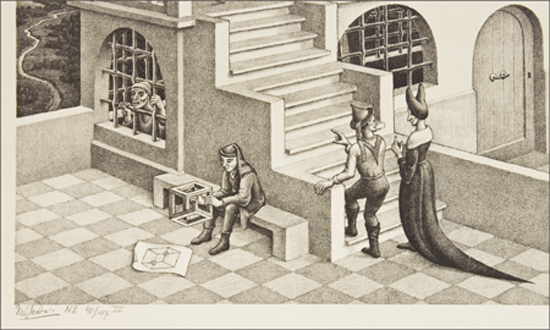
\includegraphics[width=9cm]{Belweder2.jpg}}
    \caption{Źródło: \url{www.artistmarket.com} [Dostęp: 14.06.19]}
    \end{figure}


\textit{Belweder} Eschera tworzy niezwykły świat percepcyjny będący karykaturą świata rzeczywistego. Artysta celowo deformuje świat przedstawiony aby wywołać reakcje widza, który nie jest przyzwyczajony do spostrzegania figur niemożliwych w świecie rzeczywistym. Na obrazie można dostrzec  wiele inskrypcji złożonych tworzących różne etykiety, np. czarne i białe kwadraty na parkiecie budujące podłogę, linie i krawędzie będące budulcem każdej występującej figury niemożliwej. Co ciekawe, wszystkie elementy obrazu rozpatrywane razem zyskują nowe znaczenie. Widoczne na obrazie schody spostrzegane oddzielnie nic nam o sobie nie mówią, poza tym, że są schodami niemożliwymi, ale wewnątrz świata widnieją jako schody domu. Podobnie kolumny, drabina i sześcian Neckera trzymany przez mężczyznę. Escher pozwala widzom spostrzegającym obraz  dobudować własne rozumienie przedstawionej sytuacji.   


 Escher wykorzystywał również \textit{Schody Penrose'a} na przykład na obrazie \textit{O Wchodzeniu i Schodzeniu} \citep[s. 147]{Locher}. Na szczycie przedstawionej budowli widzimy stopnie ułożone w okrąg. Wchodząc po tych stopniach ulega się iluzji ruchu, ponieważ próbując wejść na szczyt schodów, dochodzimy wciąż do tego samego miejsca z którego wyszliśmy. Wędrówka ta prowadzi nas donikąd pomimo tego, że każdy kolejny stopień schodów znajduje się wyżej od poprzedniego i teoretycznie powinniśmy wznosić się coraz wyżej. Są to zatem schody niemożliwe, których istnienia nie da się racjonalnie wyjaśnić  (por. rys. 3.5) \citep[s. 31-33]{Penrose1958}.

\begin{figure}[H]
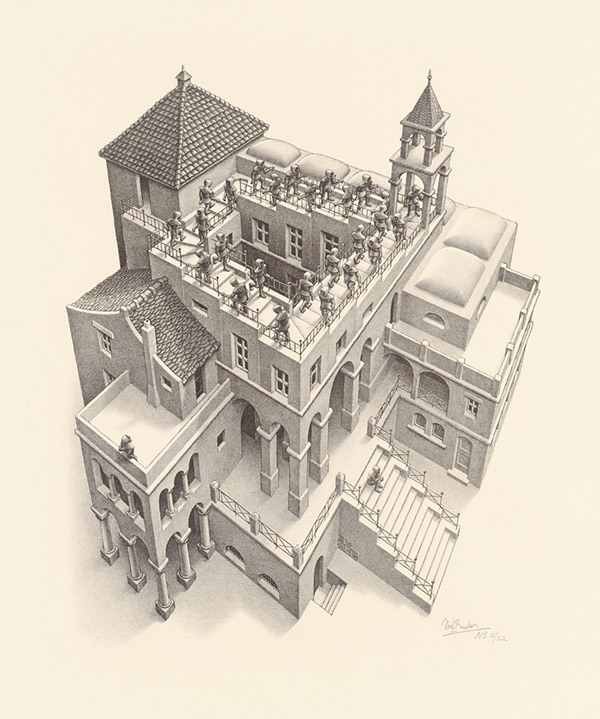
\includegraphics[width=0.8\textwidth]{ascending.jpg}
\centering
\caption{M.C Escher O Schodzeniu i Wchodzeniu, (1960) Źródło: \url{https://www.mcescher.com/gallery/recognition-success/ascending-and-descending/}}
\end{figure}


















\chapter*{Zakończenie}

Wieloznaczność według Semira Zekiego to zdolność nadawania wielu równorzędnych znaczeń spostrzeganym obiektom \citep{Wieloznacznosc}. Wieloznaczność w dziele sztuki może występować na wiele sposobów. Można zaprezentować wieloznaczność jako sytuację wyboru pomiędzy dwoma jednakowo wartościowymi perceptami (figury bistabilne) albo jako niemożność określenia istoty tego co spostrzegamy (figury iluzyjne). Według Ramachandrana i Hirsteina rolą dzieła sztuki jest wywołanie emocji estetycznej. Sądzą oni, że artyści specjalnie modyfikują swoje dzieła, aby wzmocnić w ten sposób ich cechy charakterystyczne, których wyolbrzymienie ma spowodować powstanie reakcji estetycznej \citep{Rama}.

Kontrastujące z neuroestetycznym podejście fenomenologiczne skupia się na opisie tego czym jest dzieło sztuki zamiast naukowego wyjaśnienia. Próbuje ono w sposób nowatorski i obiektywny zgłębić naturę dzieła sztuki. Widać to na przykładzie koncepcji Romana Ingardena, który proponuje rozróżnić treść przedstawioną na obrazie od tworzywa na jakim powstało. W przeciwieństwie do tradycyjnej perspektywy nie patrzy on na obraz jak na monolit, ale jak na dwie odrębne, lecz dopełniające się części. Ingarden twierdzi także, że interpretacja obrazu nie jest czynnością bierną, ale czynną wymagającą od odbiorcy twórczego zaangażowania \citep{Ingarden1958}.

Drugi rozdział pracy przedstawia stan badań nad iluzjami wzrokowymi. Omówiono ich typologię, wpływ na układ percepcyjny oraz podano przykłady różnych rodzajów iluzji często występujących w sztuce.

Ostatni rozdział przedstawia przykłady wykorzystania iluzji w pracy artystycznej holenderskiego grafika Mauritsa Cornelisa Eschera. Escher jest przykładem artysty, który postanowił zgłębić tajemnice ludzkiego wzroku za pomocą sztuki. Wykorzystuje on malarstwo do zaskakiwania widza poprzez użycie złudzeń optycznych. Sensem sztuki Eschera jest zniekształcanie rzeczywistości w taki sposób żeby skłonić odbiorce sztuki do zadawania pytań odnośnie rzeczywistej treści własnych spostrzeżeń \citep{Locher}. Escher jest także jednym z prekursorów sztuki matematycznej, pozwala on nam odkryć niedostrzegane wcześniej piękno matematyki. Analiza dzieł Eschera została przeprowadzona w oparciu o trójpoziomowy semiotyczny model dzieła sztuki Moniki Bianki Florek. Każdy z zaprezentowanych obrazów składa się z trzech niezależnych warstw, które wzajemnie się przenikając tworzą doświadczenie estetyczne widza. Oglądanie dzieł Eschera nie jest tylko bierną percepcją zawartej na nich treści. Zrozumienie znaczenia obrazu i tego z czego jest zbudowany wymaga nie lada wysiłku i twórczej kreatywności, która musi wykazać się odbiorca dzieła chcąc odkryć znaczenie obrazu.




 \addcontentsline{toc}{chapter}{Zakończenie}
 



















































% Spis rysunków (jeżeli jest potrzebny):
%\listoffigures

%
% Literatura:
\bibliography{bib}
\addcontentsline{toc}{chapter}{Bibliografia}
%
% Spis tabel (jeżeli jest potrzebny):
%\listoftables
%
%
% Skorowidz (opcjonalnie)
%\printindex



\end{document}
